\documentclass[a4paper]{cours-bdd}

\cristal

\title{COVID Simulation}

\begin{document}

\frame{\titlepage}


% --------------------------------------


\begin{frame}
  \hfill \
  \begin{center}
    \Huge
    Préambule
  \end{center}
  \hfill \

\end{frame}



% --------------------------------------

\begin{frame}[fragile]
  \frametitle{Modéliser les épidémies : pour faire quoi ?}

  Aider à comprendre.\\
  Aide à la décision.\\
  Essayer de répondre aux grandes questions. \\
  \begin{itemize}
  \item Combien de temps va durer l’épidémie ?
  \item Combien de personnes seront infectées au cours de la crise ? 
  \item Combien de personnes décèderont au cours de la crise ? 
  \item Combien de personnes doivent être immunisées ?
  \item Quand mettre en place un ou des confinements ?
  \item Quelle durée doivent avoir les confinements ?
  \item Quand arrivera t-on à saturation des hopitaux ?
  \end{itemize}
  
\end{frame}

  
% --------------------------------------

\begin{frame}[fragile]
  \frametitle{Différentes approches}

  %\fbox{}
  \begin{minipage}[b]{0.45\columnwidth}
    \vspace{0.0cm}
    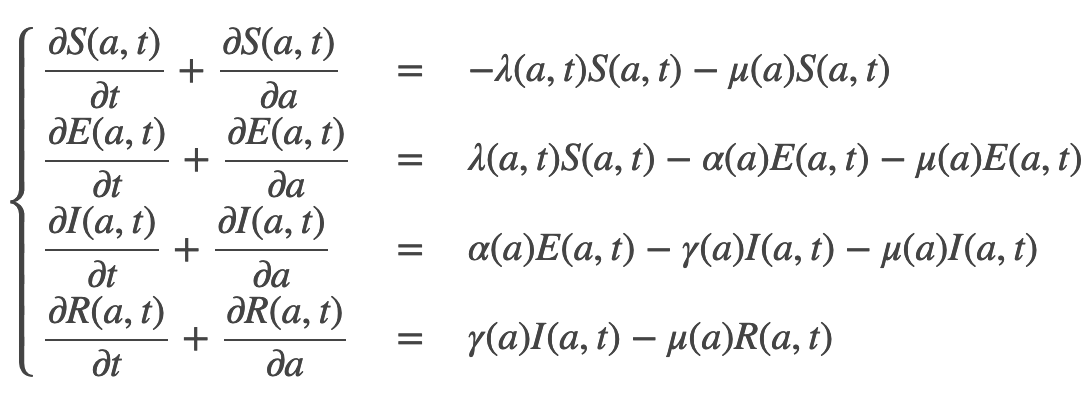
\includegraphics[width=\linewidth]{approcheMath.png} \\
    Approche Mathématique 
      \end{minipage}    
  \hfill \ 
  \begin{minipage}[b]{0.45\columnwidth}
        \vspace{0.0cm}
        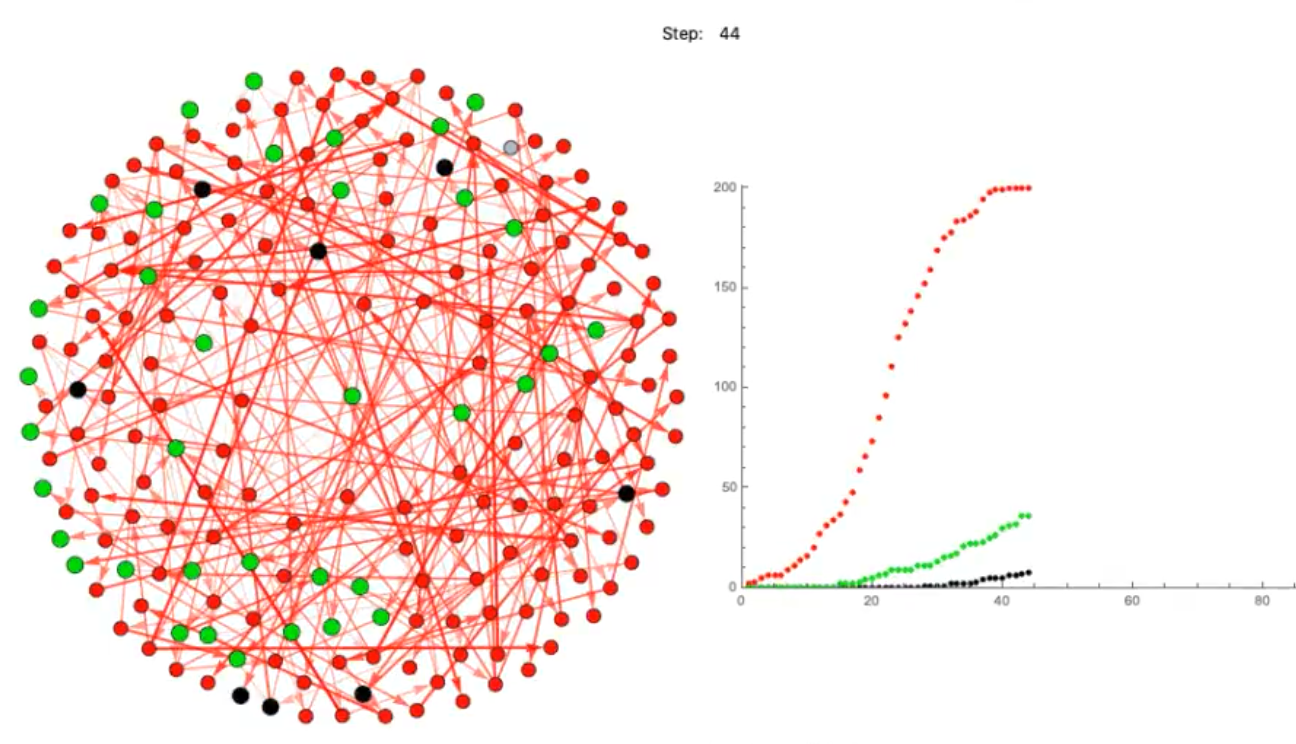
\includegraphics[width=0.8\linewidth]{approcheNetwork.png} \\
        Approche par réseaux sociaux
      \end{minipage}
      \ 

  \begin{minipage}[t]{0.45\columnwidth}
        \vspace{0.0cm}
        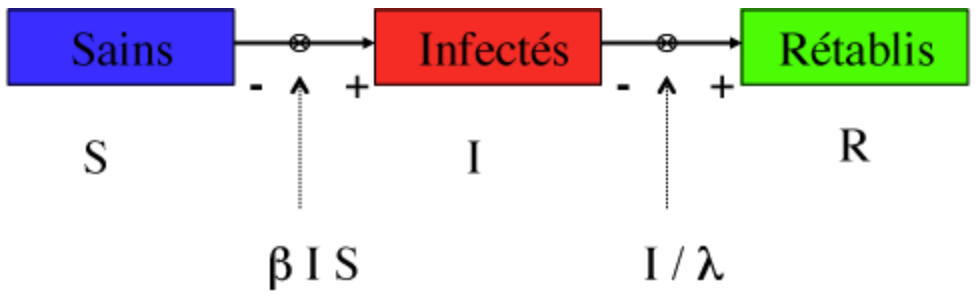
\includegraphics[width=\linewidth]{modeleSIR.png} \\
        Approche par flux
  \end{minipage}
  \hfill \
  \begin{minipage}[t]{0.45\columnwidth}
        \vspace{0.0cm}
        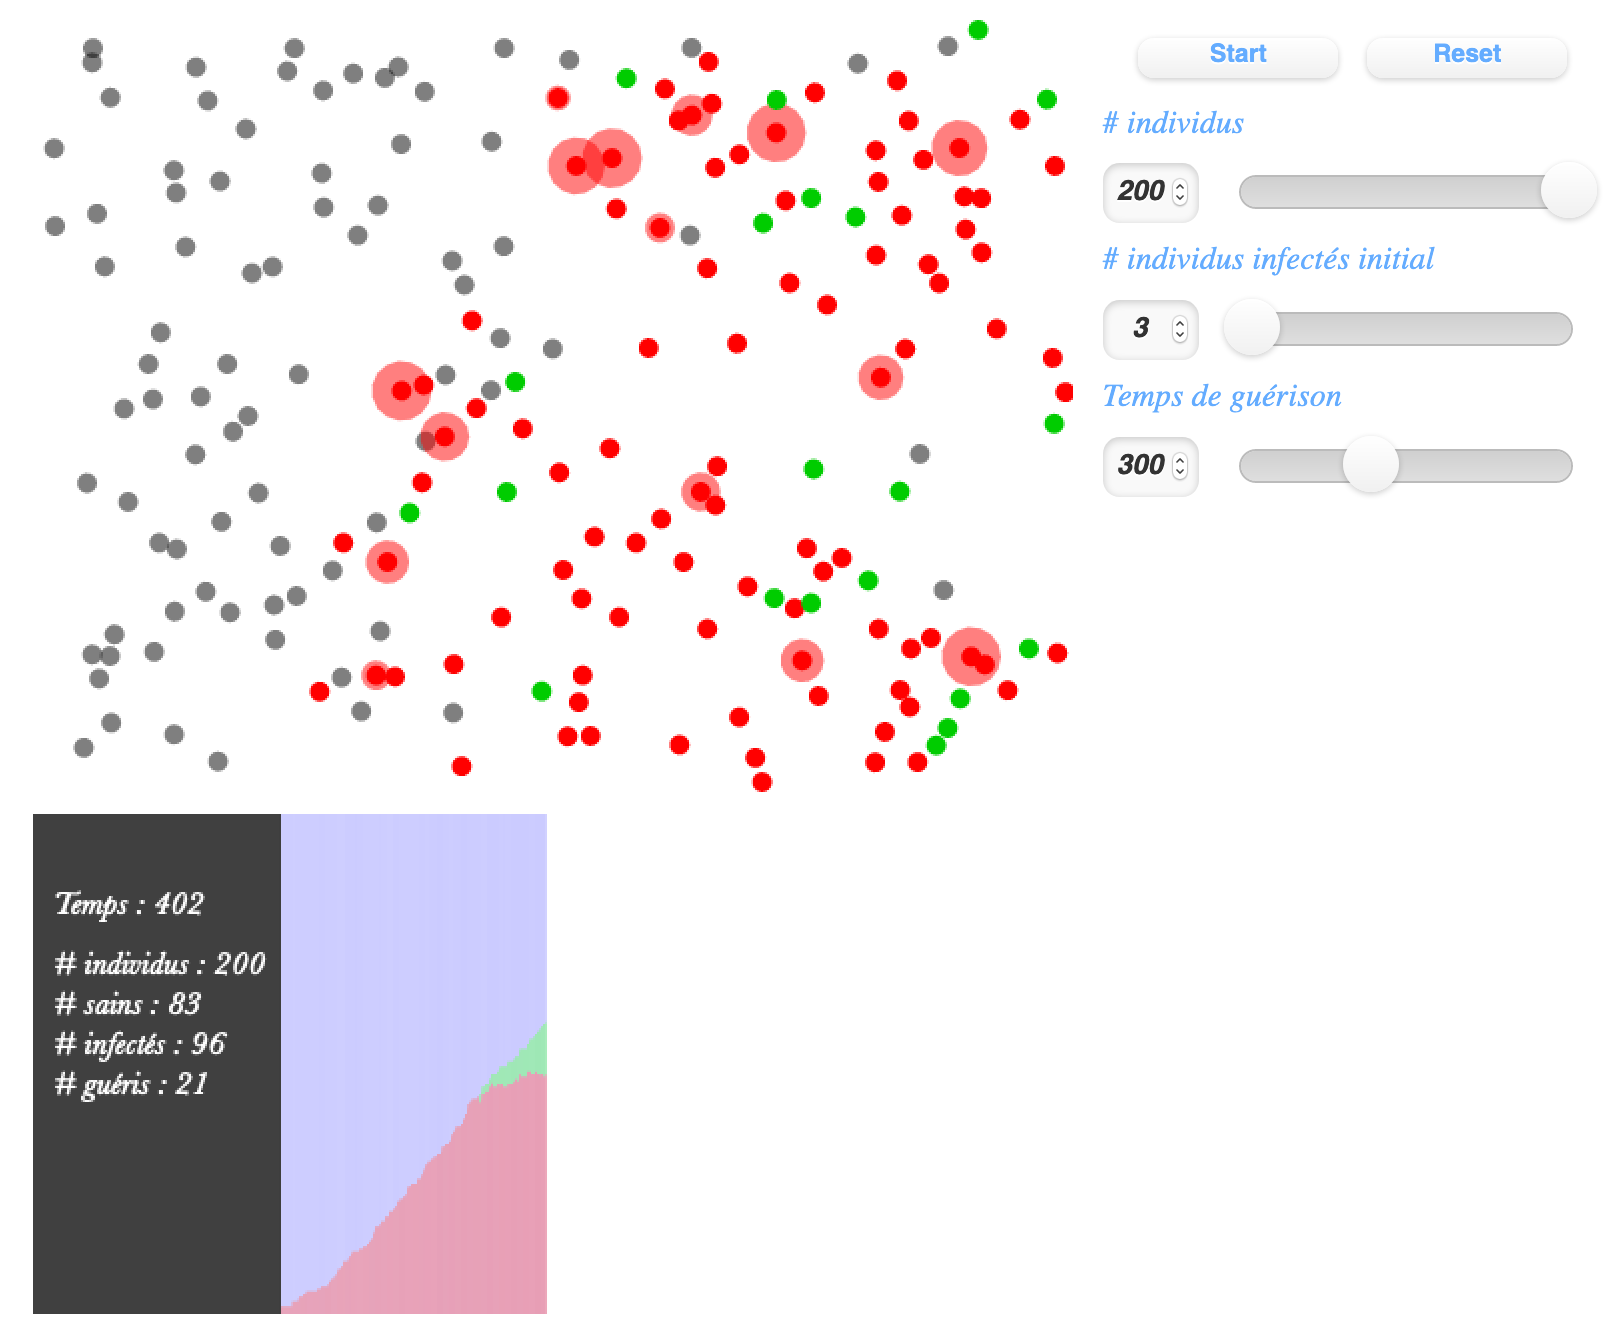
\includegraphics[width=0.6\linewidth]{approcheSMA.png} \\
        Approche centrée individus
  \end{minipage}
  \
  
\end{frame}

% --------------------------------------


\begin{frame}
  \hfill \
  \begin{center}
    \Huge
    Notre situation actuelle
  \end{center}
  \hfill \

\end{frame}



% --------------------------------------

\begin{frame}[fragile]
  \frametitle{Notre modèle - notre méthodologie}
  \begin{itemize}
  \item Approche par flux (compartiments) ``classique'' \\ (tout comme Inserm ou Pasteur)
    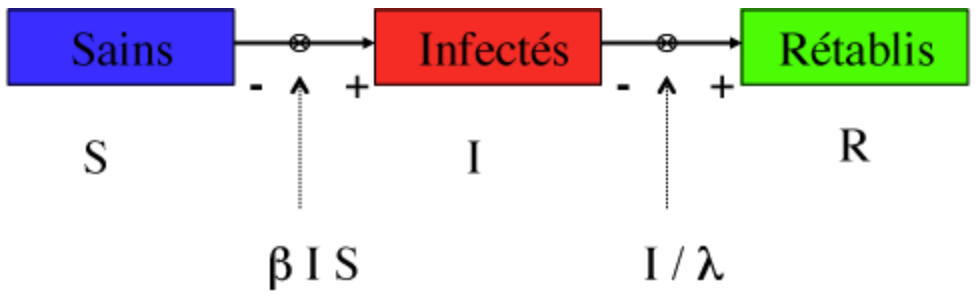
\includegraphics[width=0.6\linewidth]{modeleSIR.png} \\
  \item Prise en compte Asymptomatiques, Graves, Décès, etc ...
    
    \bigskip    
    \textbf{Points originaux:}
  % \item SIGRM avec contagiosité variable tout au long du temps
  \item Contagiosité variable tout au long du temps
  % \item SIAGRM (avec asymptomatiques et non asymptomatiques)
  \item Techniques d'IA pour identifier les bonnes valeurs des paramètres 
  \end{itemize}
  
\end{frame}



% --------------------------------------

\begin{frame}[fragile]
  \frametitle{La validation}
  \begin{itemize}
  \item Un modèle s'appuie sur des paramètres
  \item Plus il y a de paramètres plus c'est facile de coller aux données (overfitting)
  \end{itemize}

  \bigskip
  
  \textbf{Question : Comment valider le modèle}

  \begin{itemize}
  \item Par autorité
    
  \item par calibration
    \begin{itemize}
    \item Par les faits stylisés propres à une épidémie 
      (croissance exponentielle, puis décroissance)
    \item Par sa capacité à reproduire les situations passées % (est-ce qu'on peut régler les paramètres pour que le modèle montre la situation actuelle)
  \end{itemize}

  \end{itemize}
\end{frame}


% --------------------------------------

\begin{frame}[fragile]
  \frametitle{Faits stylisés}
  
  \begin{center}
            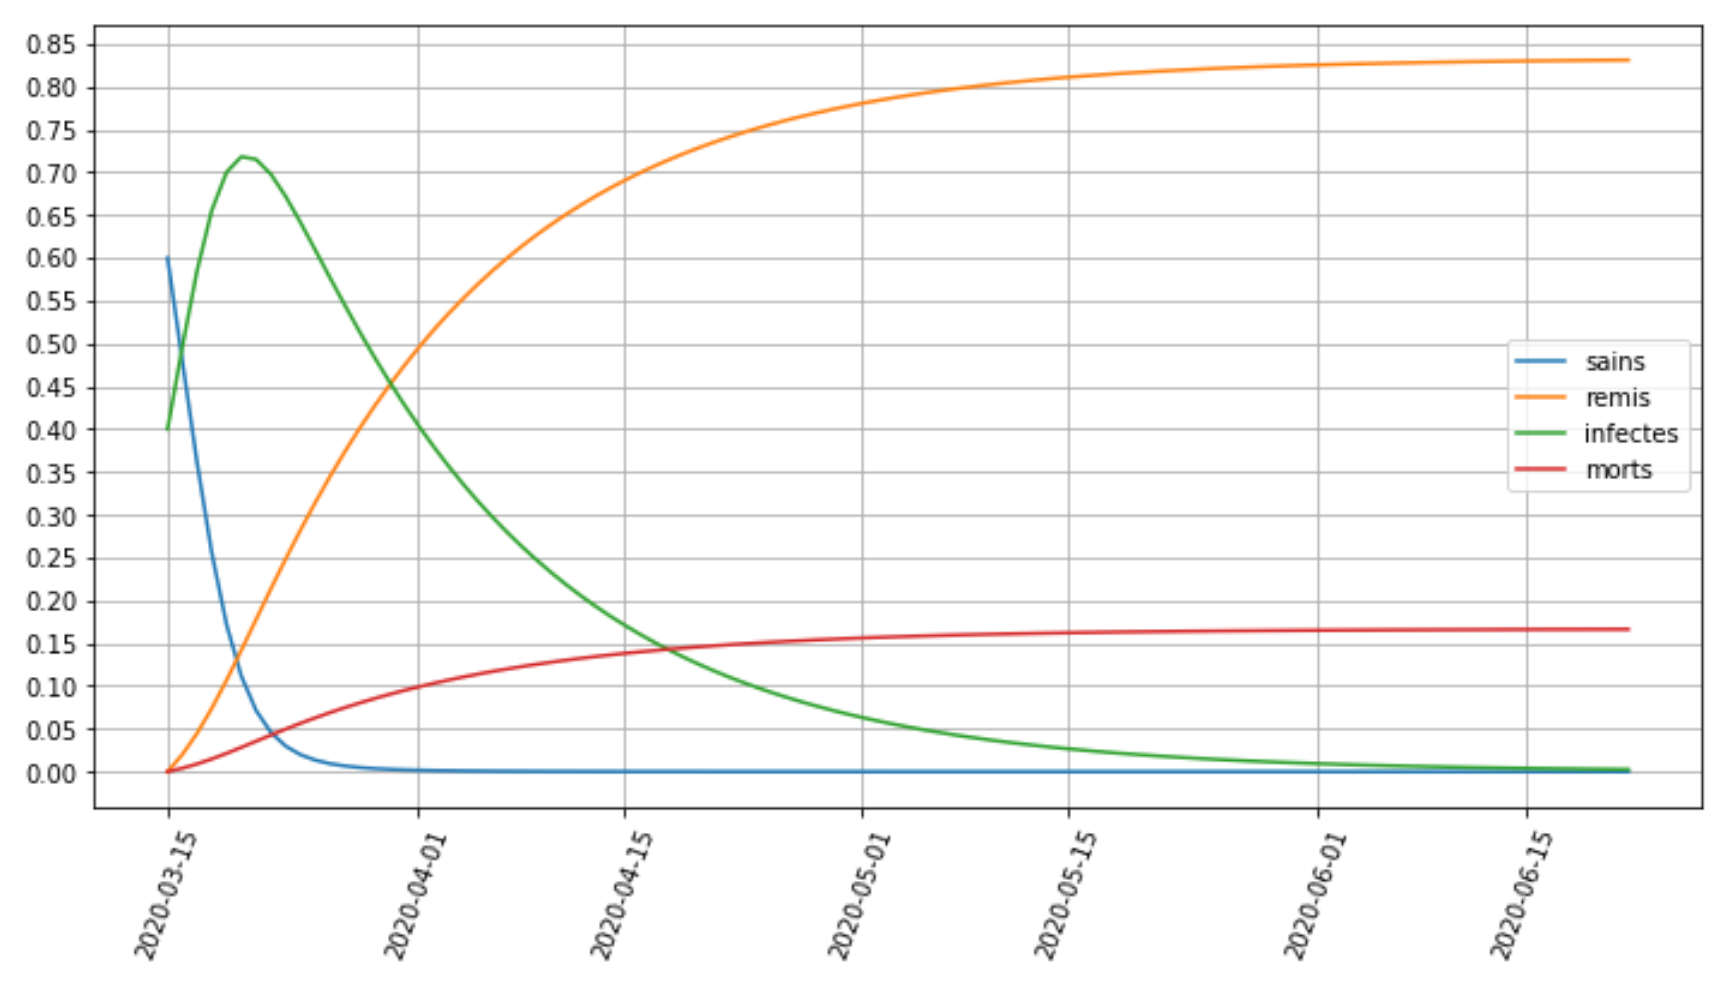
\includegraphics[width=1.0\linewidth]{fig3_sirgm.png} \\
  \end{center}

  
\end{frame}


% --------------------------------------

\begin{frame}[fragile]
\frametitle{Coller à la réalité : Réa}

  \begin{center}
    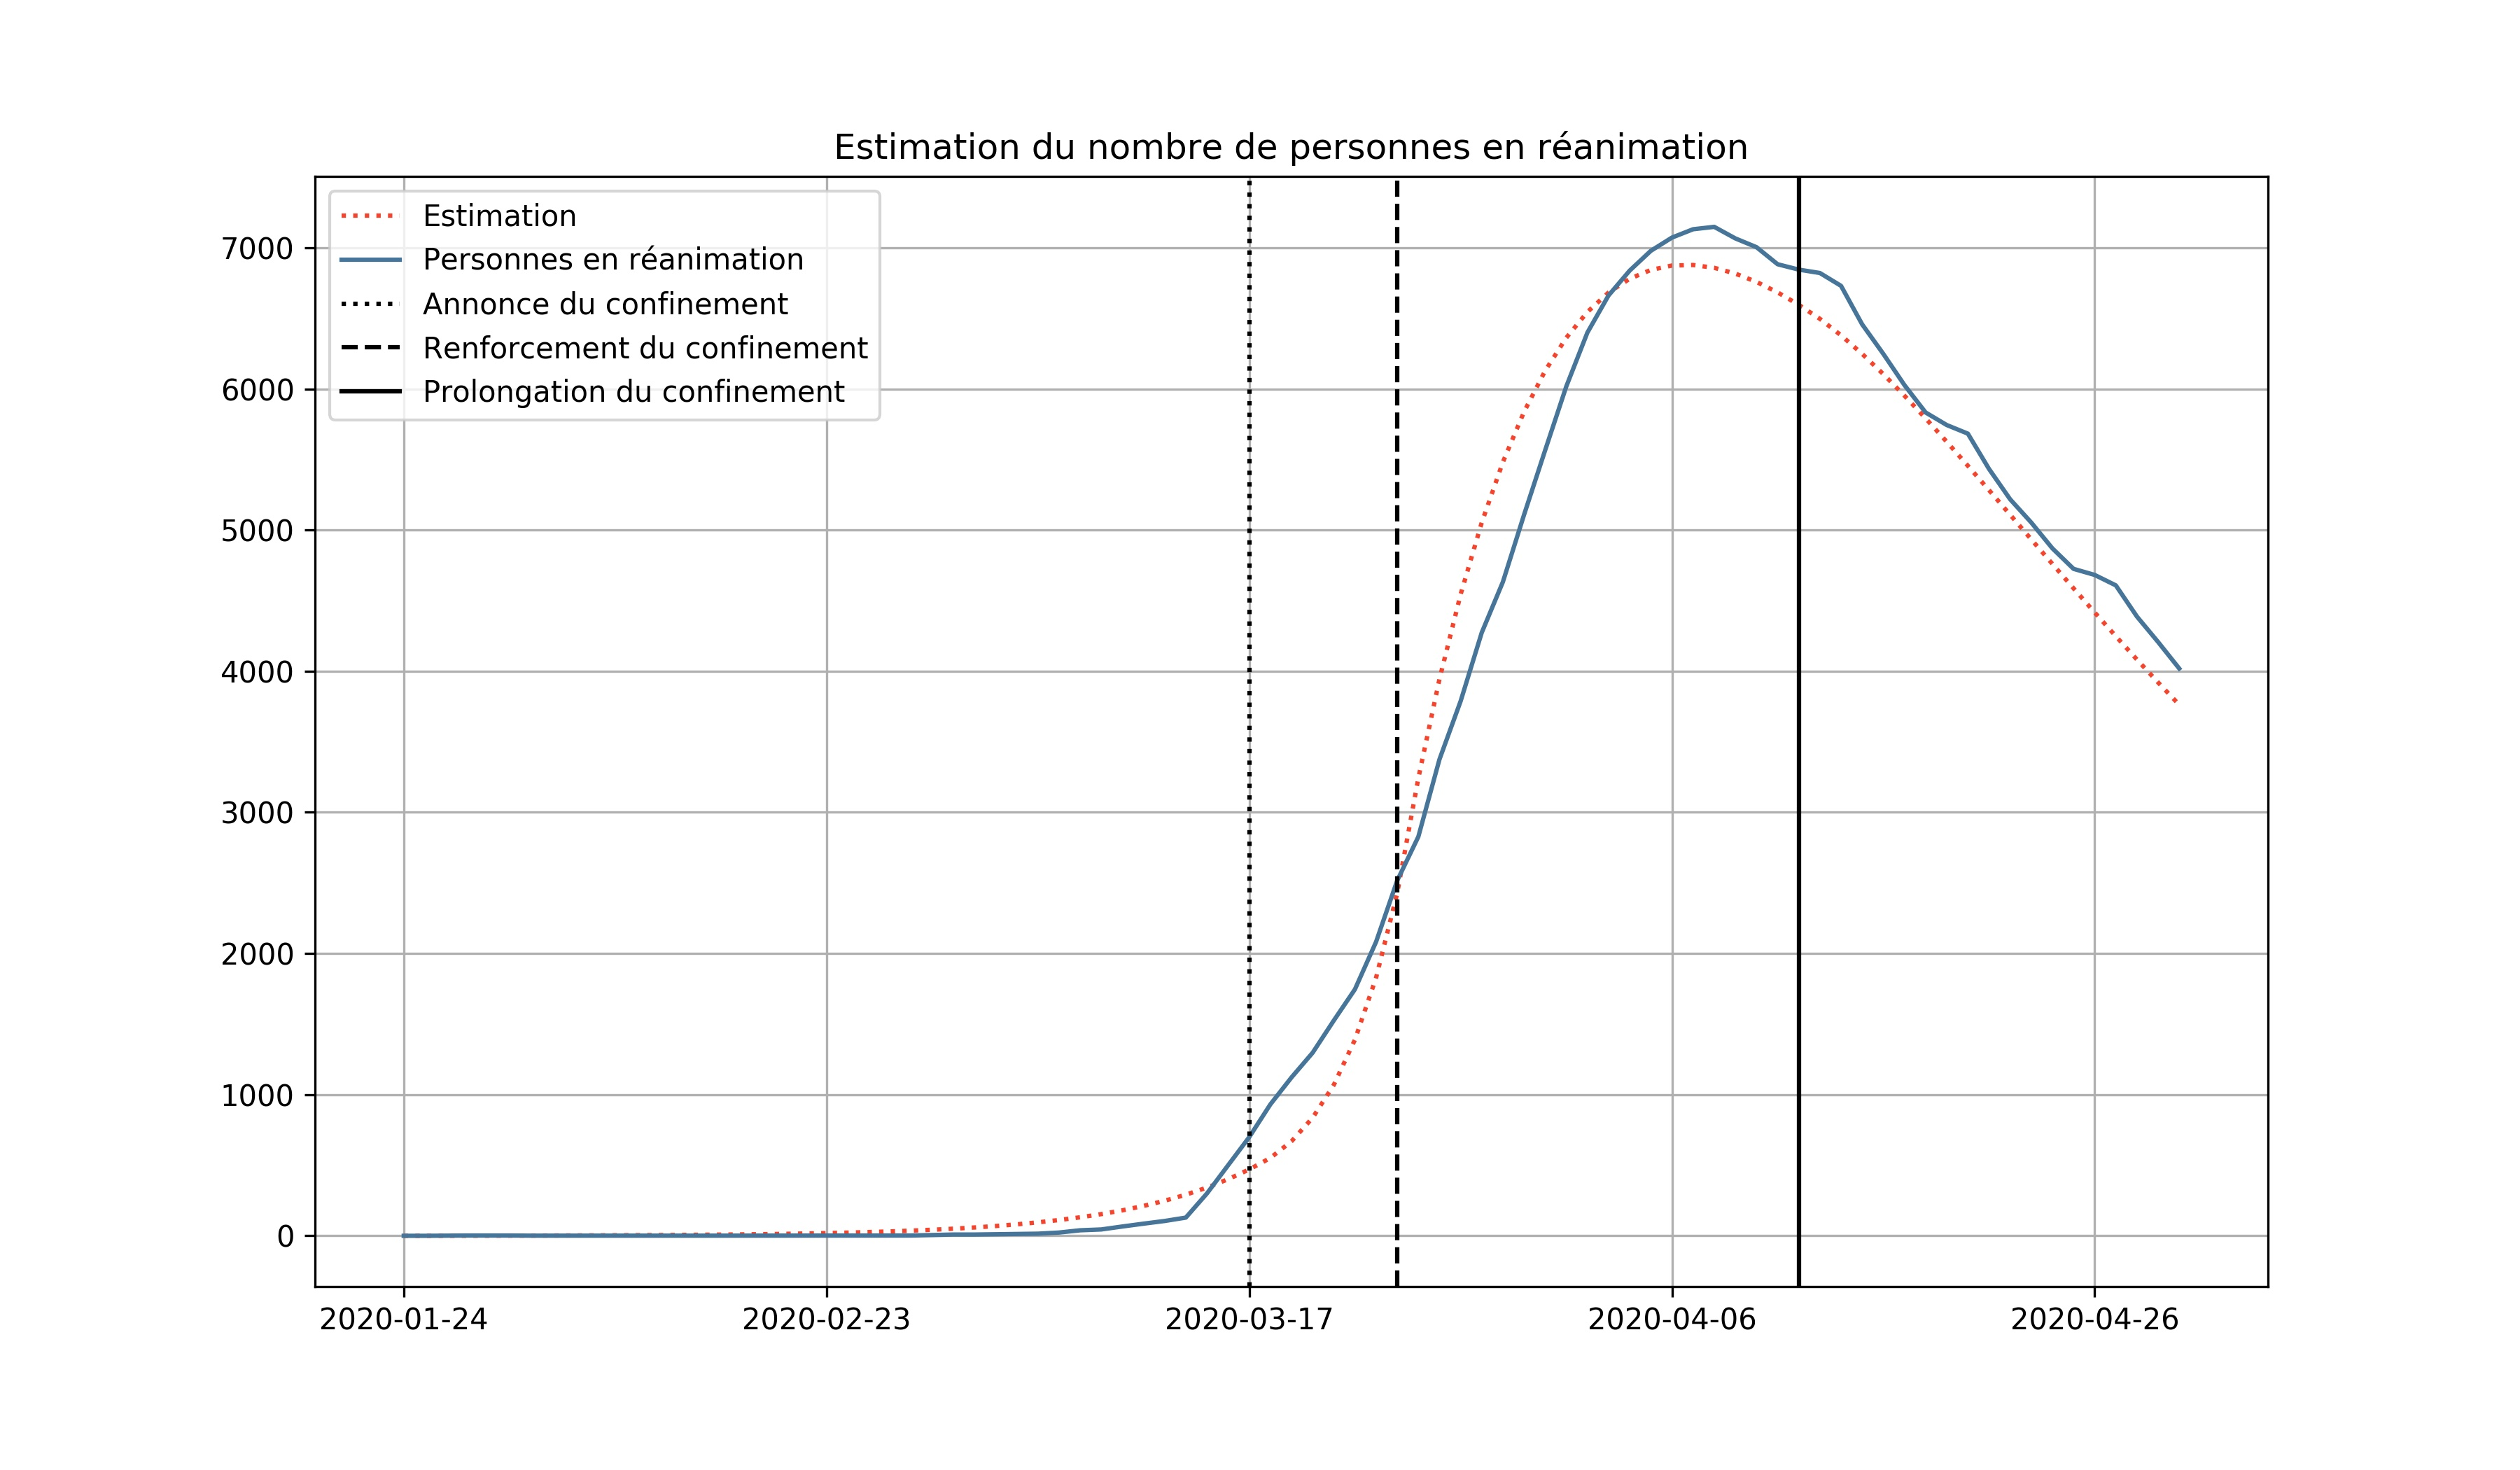
\includegraphics[width=1.0\linewidth]{figure1.jpg} \\
    {\tiny à partir des données ministère santé \texttt{data.gouv.fr}}
  \end{center}
  
\end{frame}

% --------------------------------------

\begin{frame}[fragile]
\frametitle{Coller à la réalité : Décès}

  \begin{center}
    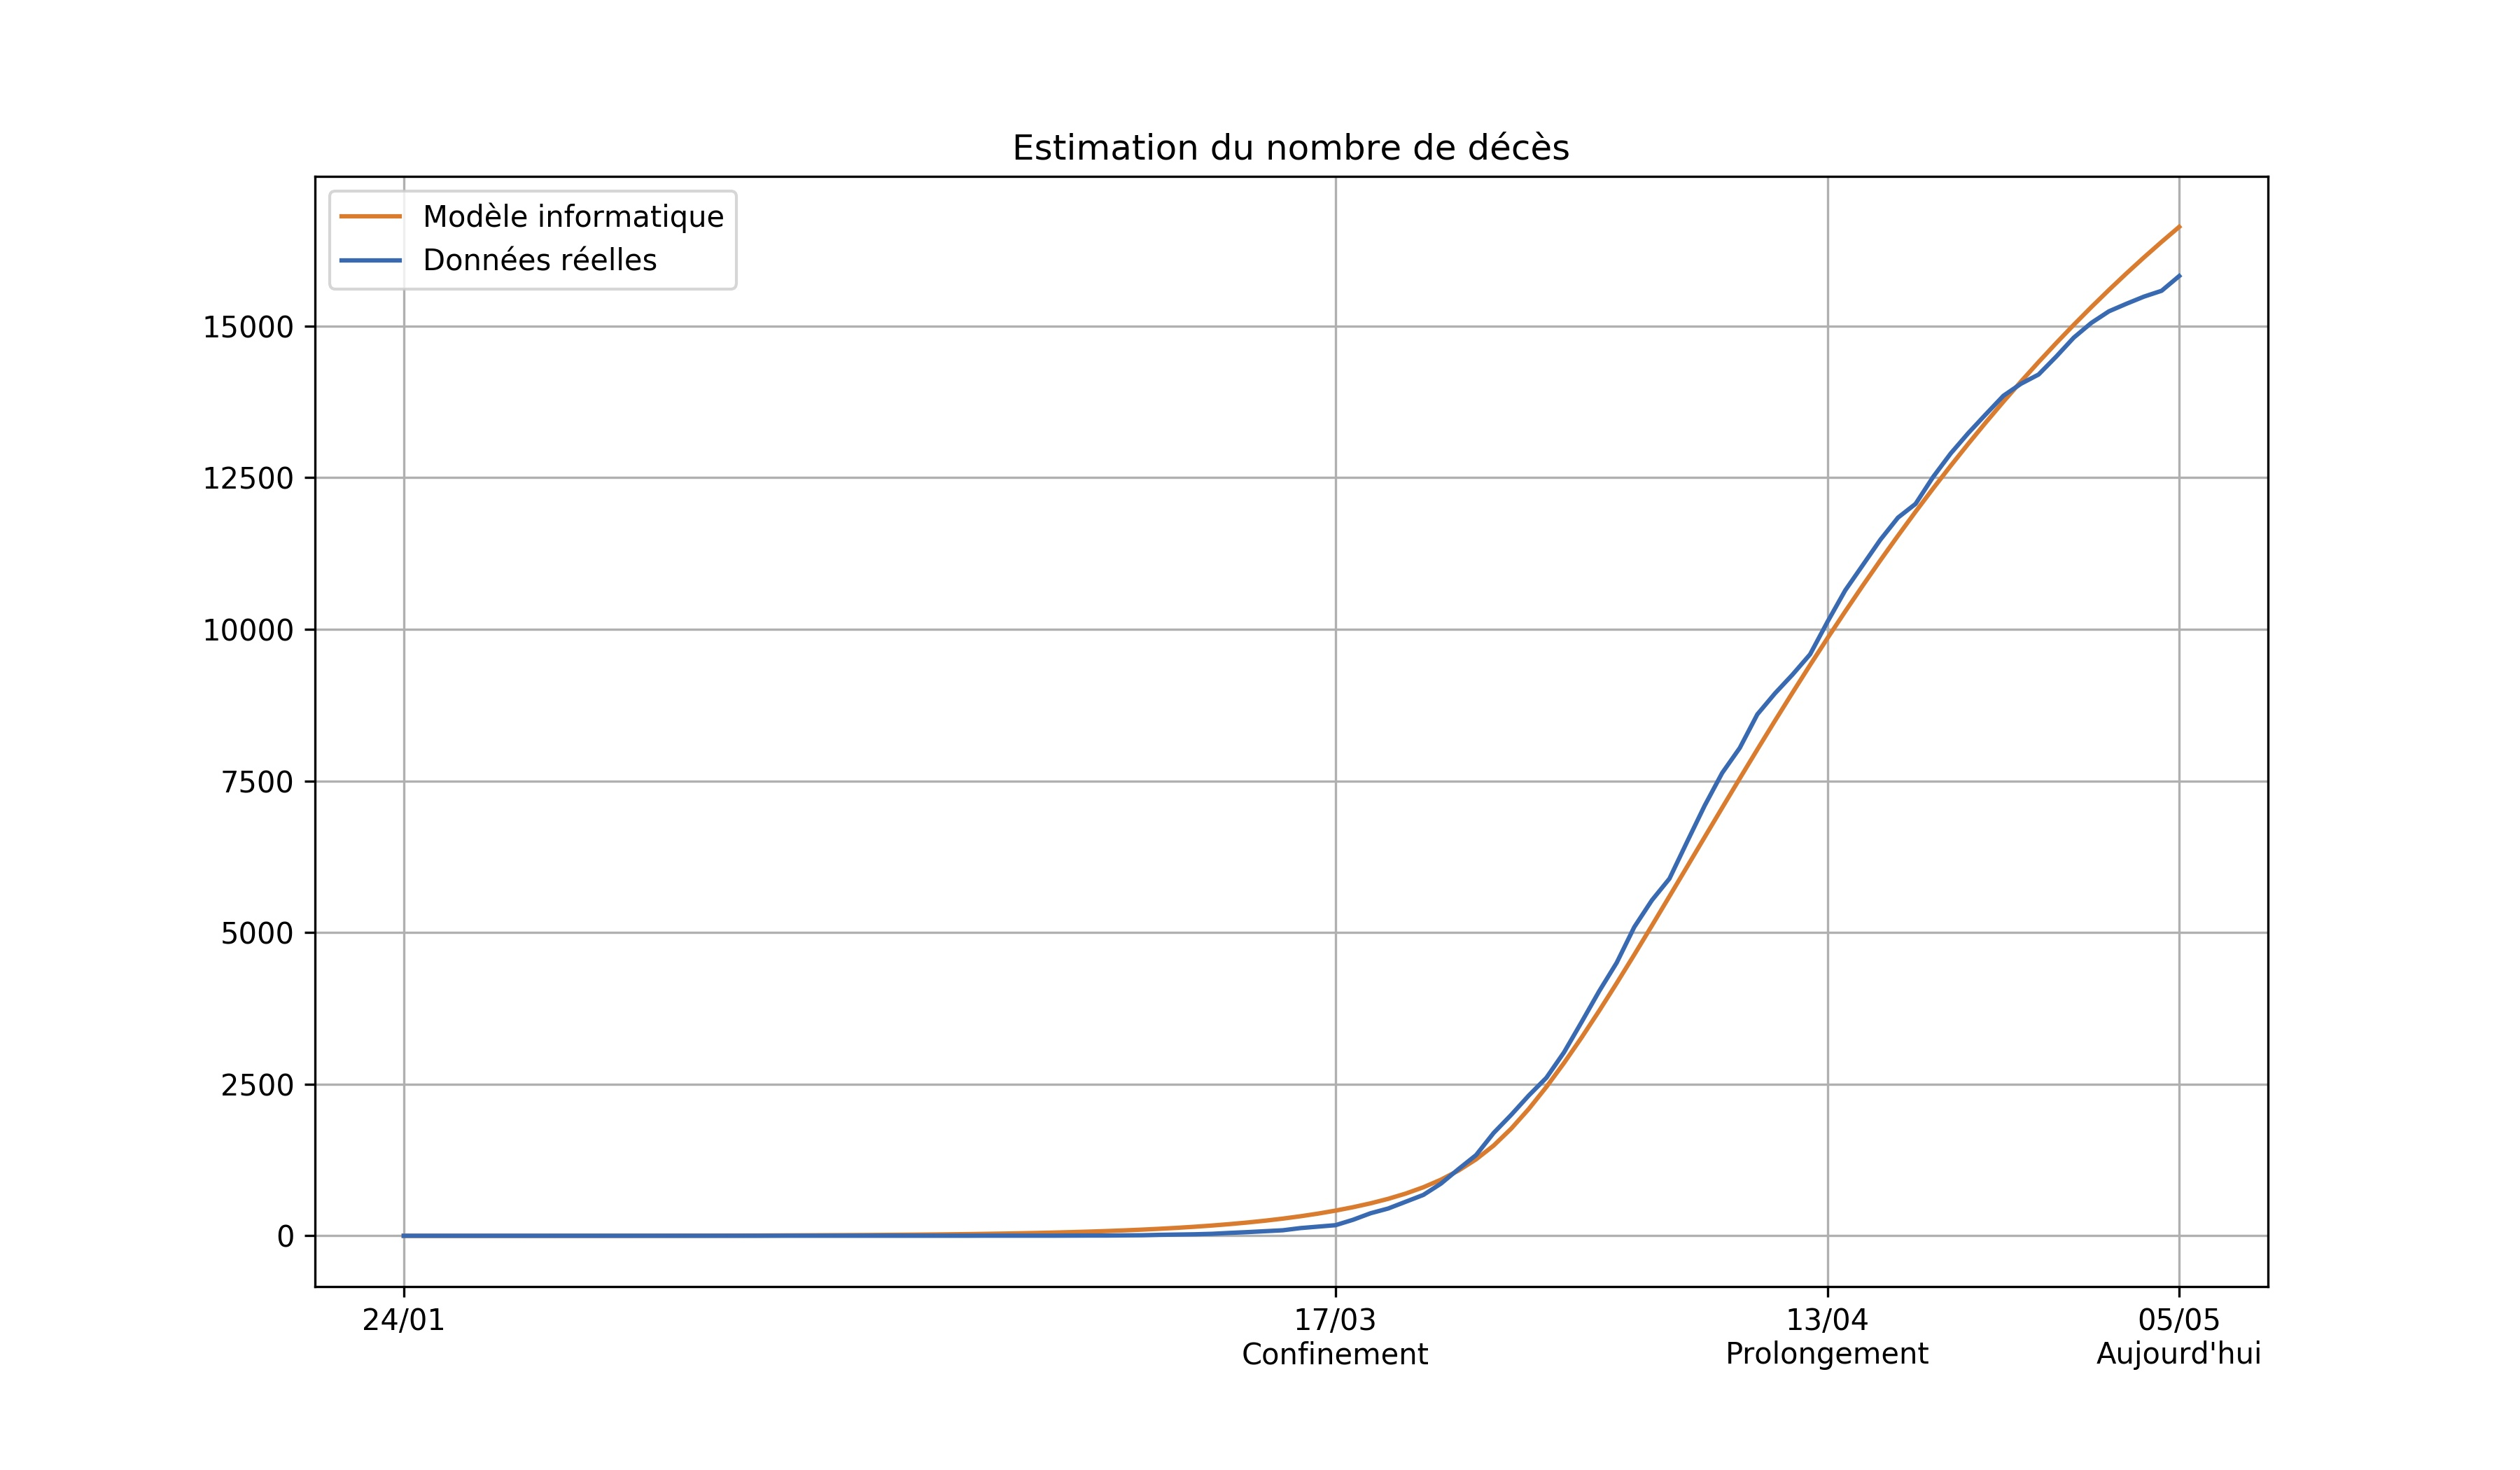
\includegraphics[width=1.0\linewidth]{figure2.jpg} \\
    {\tiny à partir des données ministère santé \texttt{data.gouv.fr}}
  \end{center}
  
\end{frame}

% --------------------------------------

\begin{frame}[fragile]
\frametitle{Projection sur Réa : 3 hypothèses}

  \begin{center}
    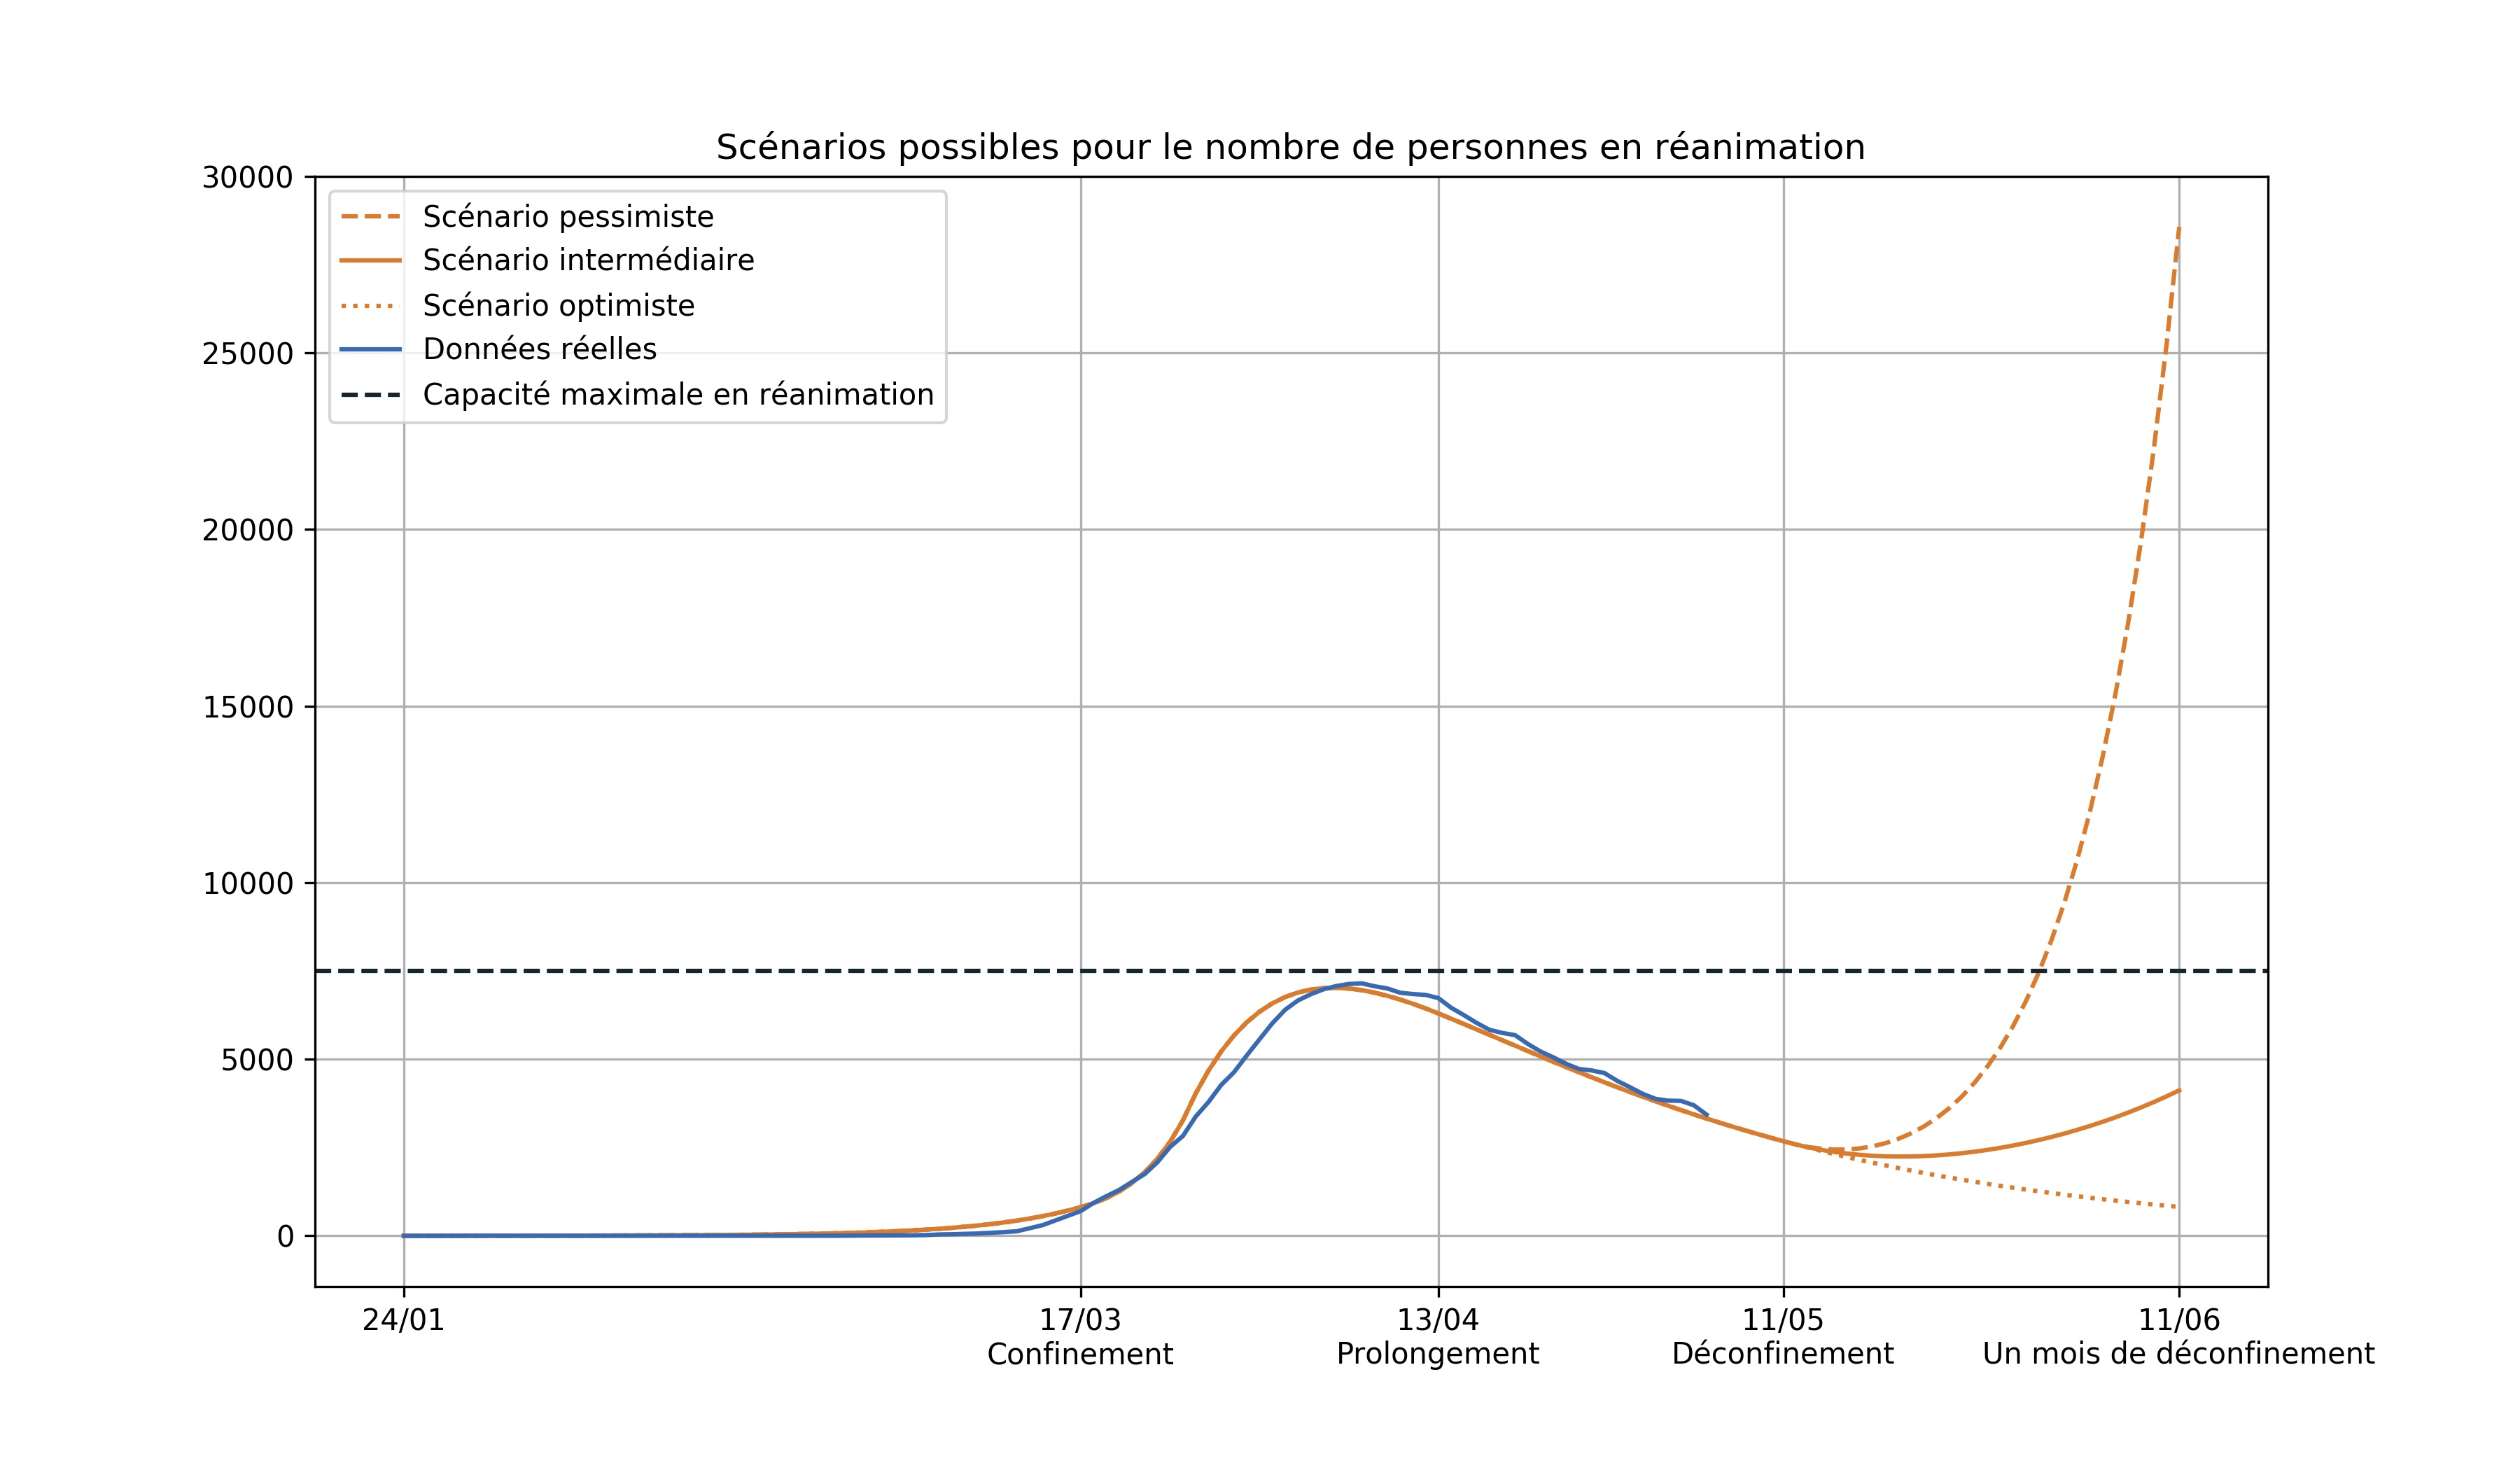
\includegraphics[width=1.0\linewidth]{figure3.jpg} \\
    {\tiny à partir des données du ministère de la santé \texttt{data.gouv.fr}}
  \end{center}
  
\end{frame}

% --------------------------------------

\begin{frame}[fragile]
\frametitle{Projection sur Décès : 3 hypothèses}

  \begin{center}
    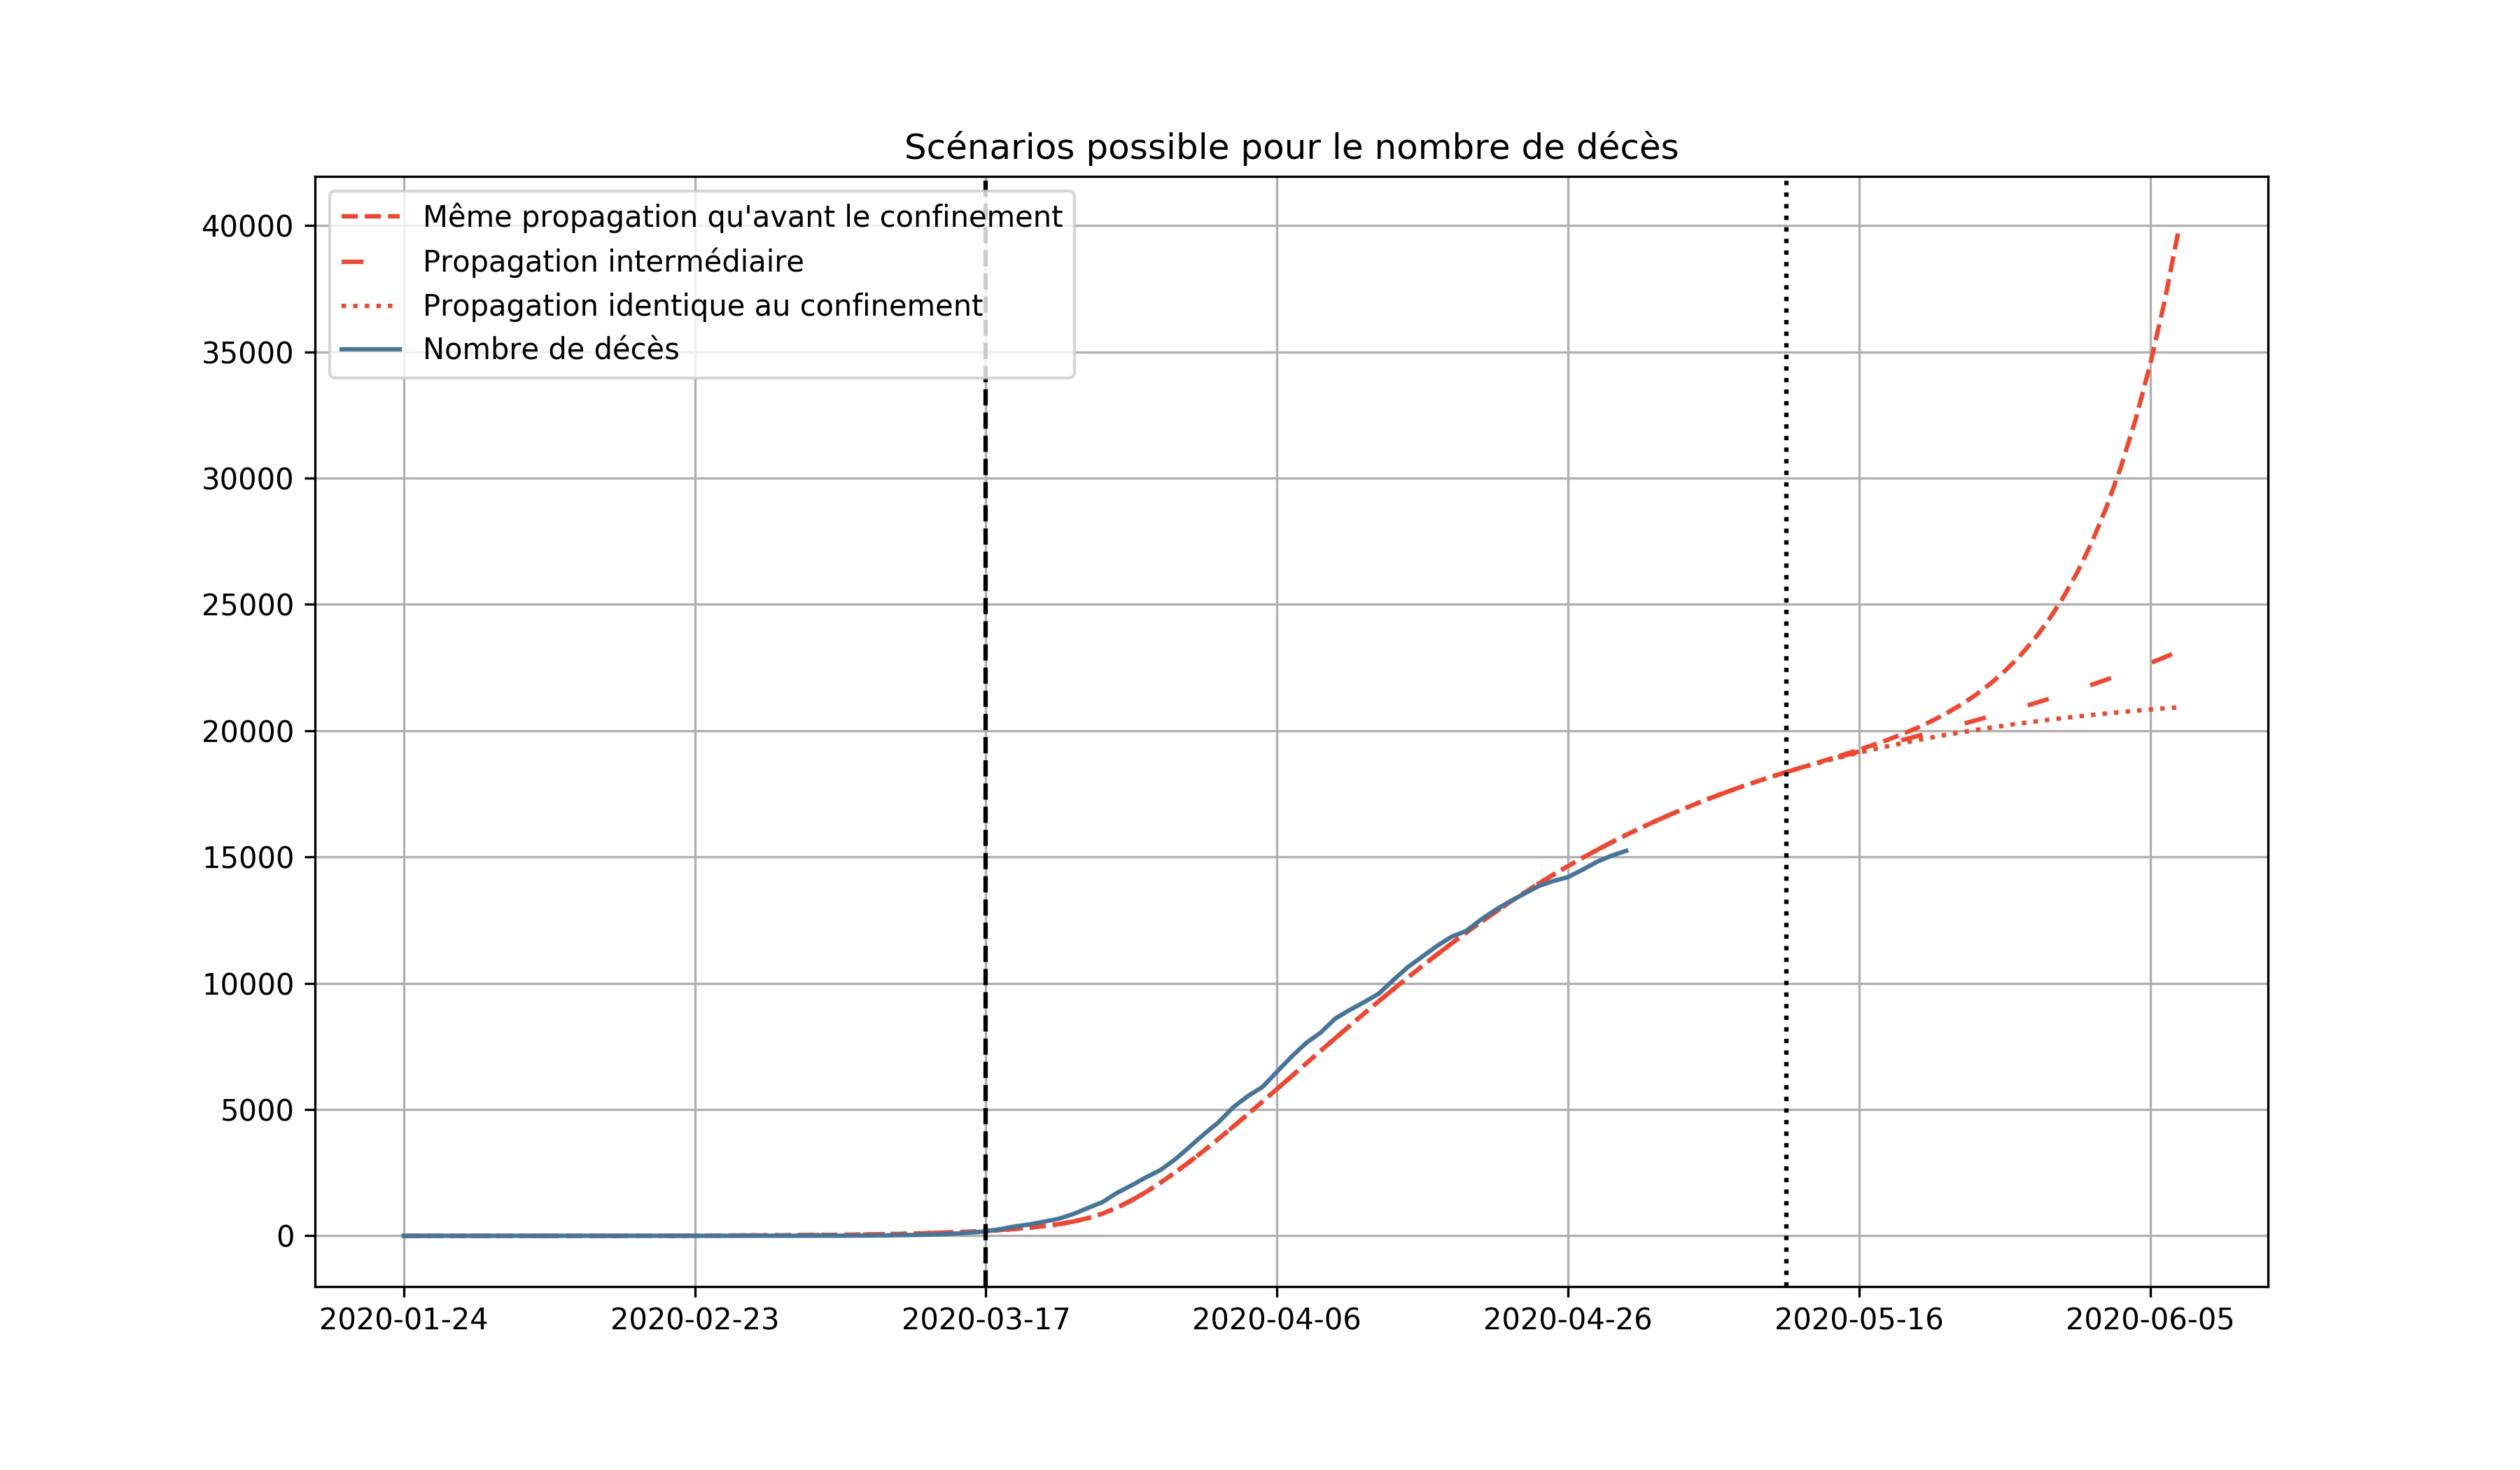
\includegraphics[width=1.0\linewidth]{figure4.jpg} \\
    {\tiny à partir des données du ministère de la santé \texttt{data.gouv.fr}}
  \end{center}
  
\end{frame}

% --------------------------------------

\begin{frame}[fragile]
\frametitle{Propagation intermédiaire : rester < 7000 lits ?}

  \begin{center}
    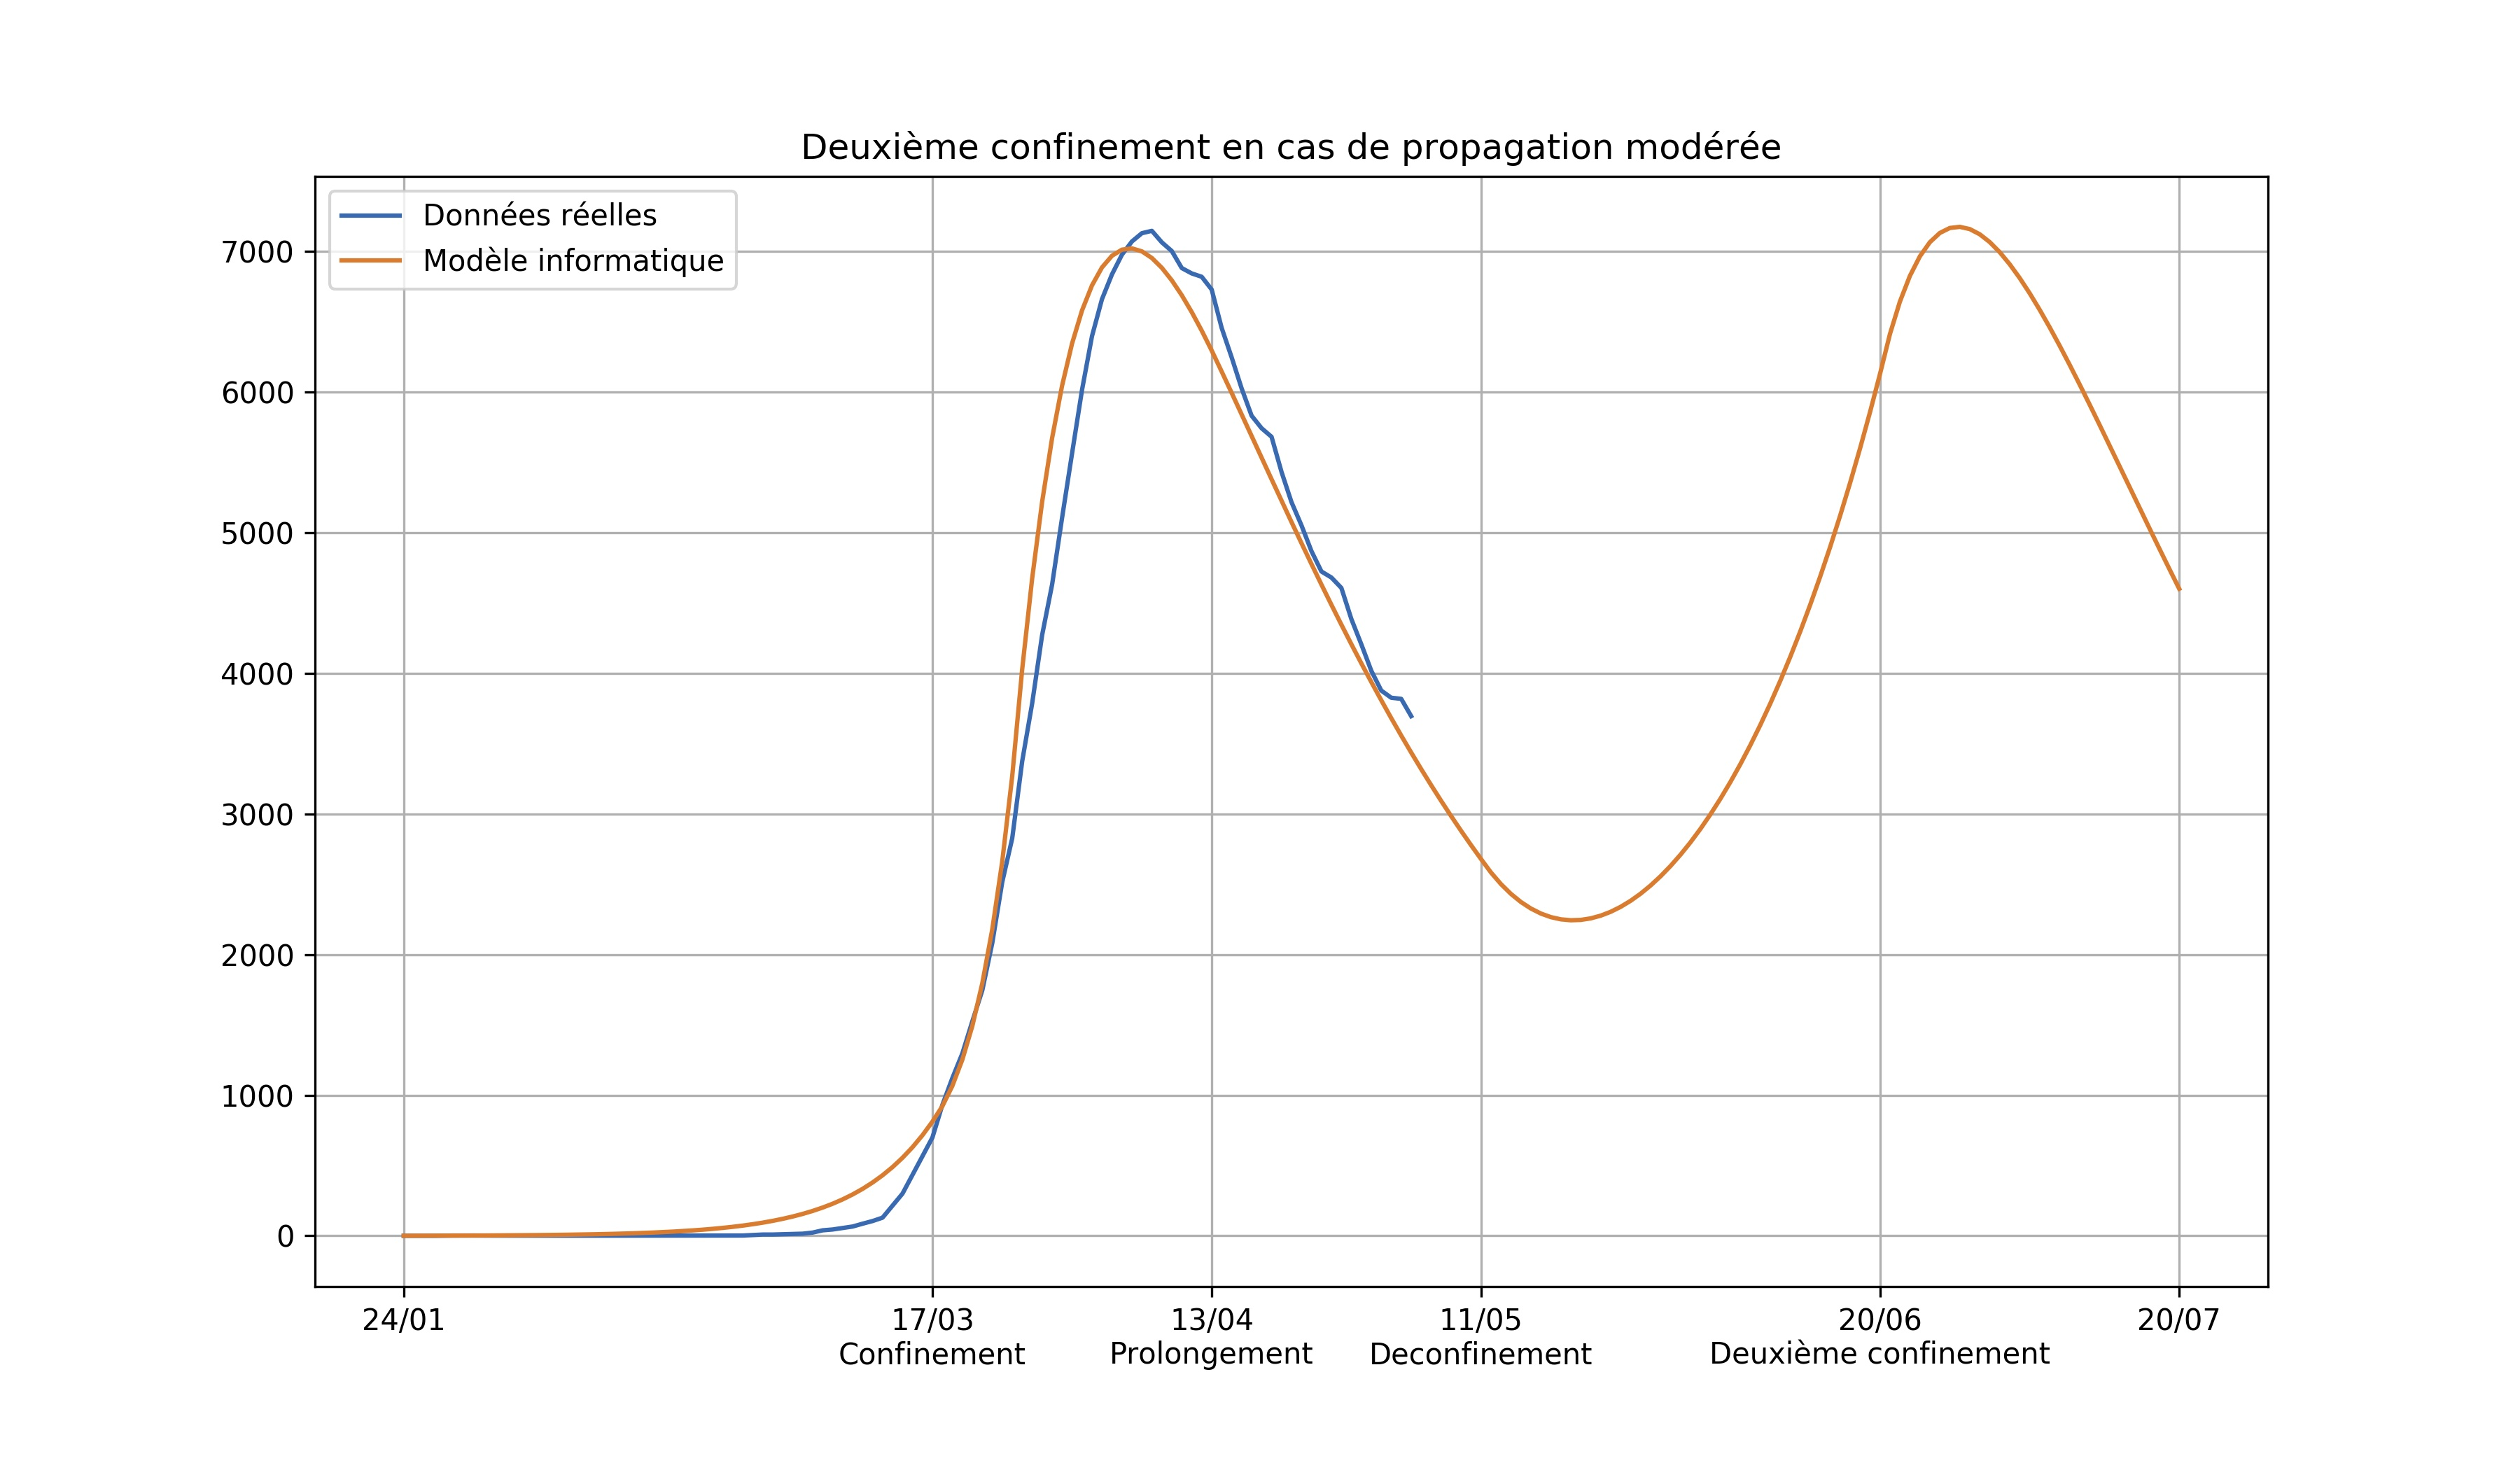
\includegraphics[width=1.0\linewidth]{figure5.jpg} \\

        \textbf{Confinement necessaire au 20 juin}
  \end{center}
  
\end{frame}

% --------------------------------------

\begin{frame}[fragile]
\frametitle{Propagation pessimiste : comment rester < 7000 lits ?}
\begin{center}
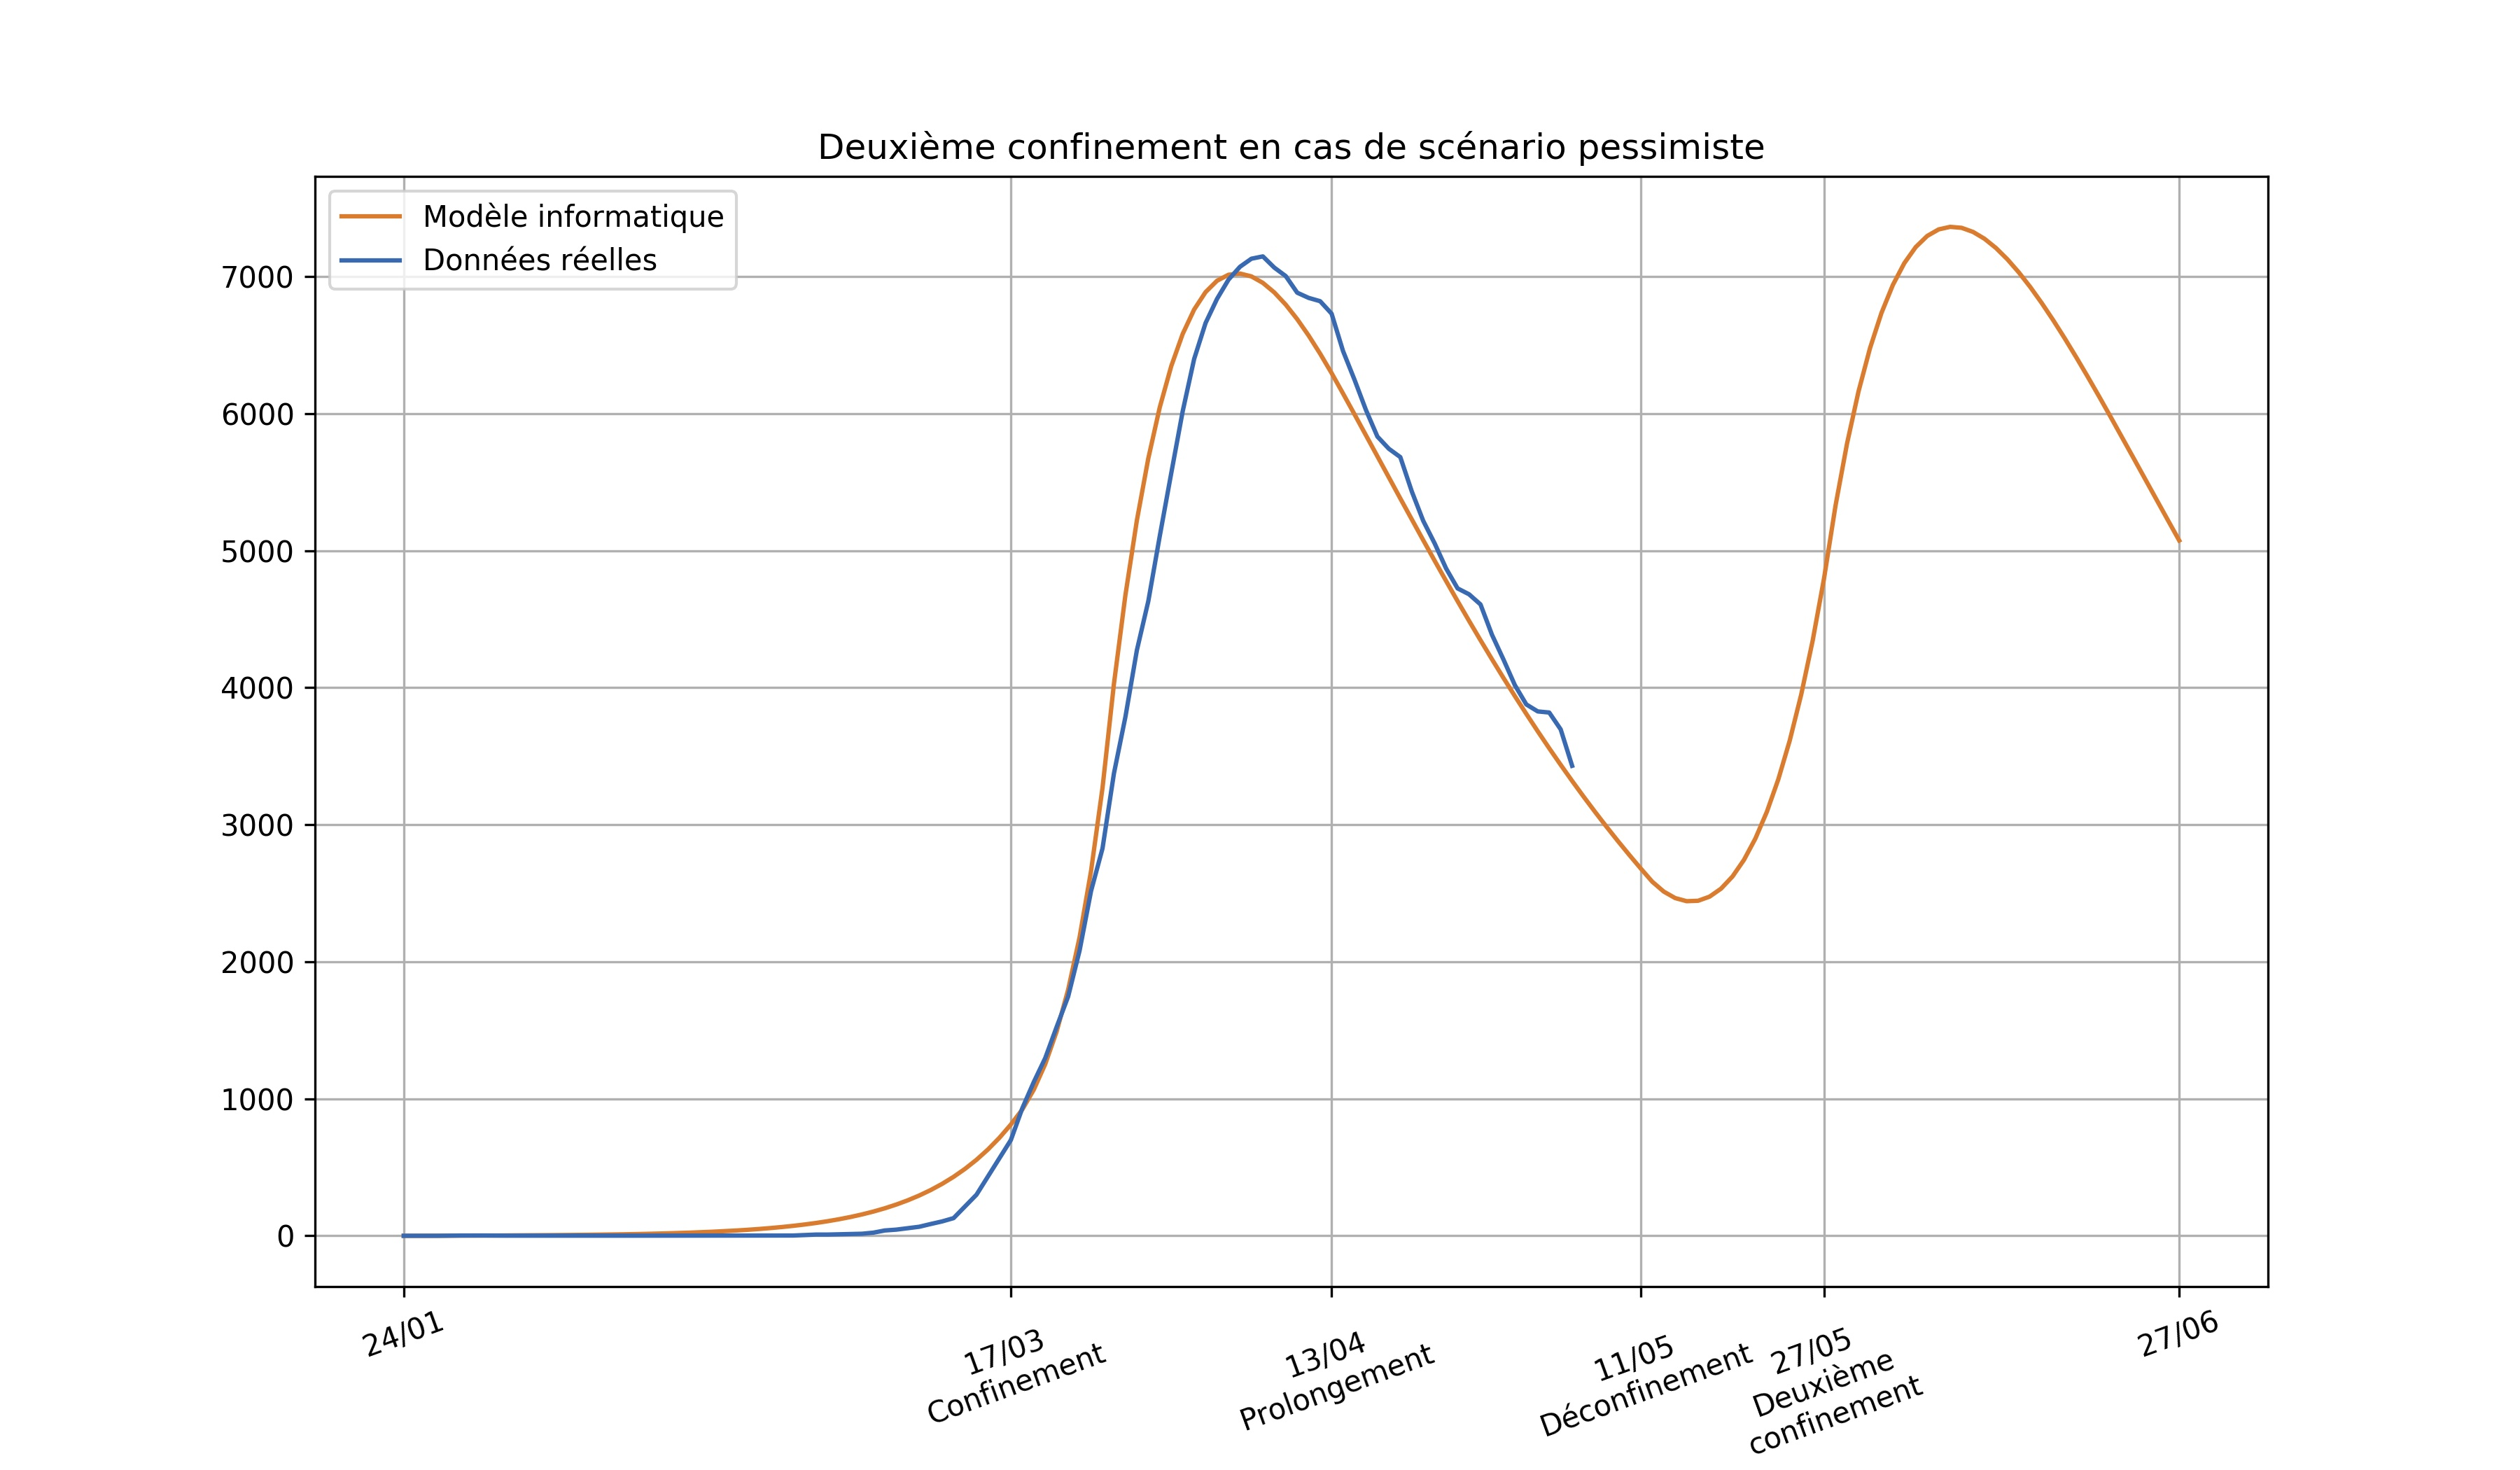
\includegraphics[width=1.0\linewidth]{figure6.jpg} \\

\textbf{Confinement nécessaire au 27 mai}

  \end{center}
  
\end{frame}

% --------------------------------------

\begin{frame}[fragile]
\frametitle{Et si on décale d'1 jour ?}

\begin{center}
    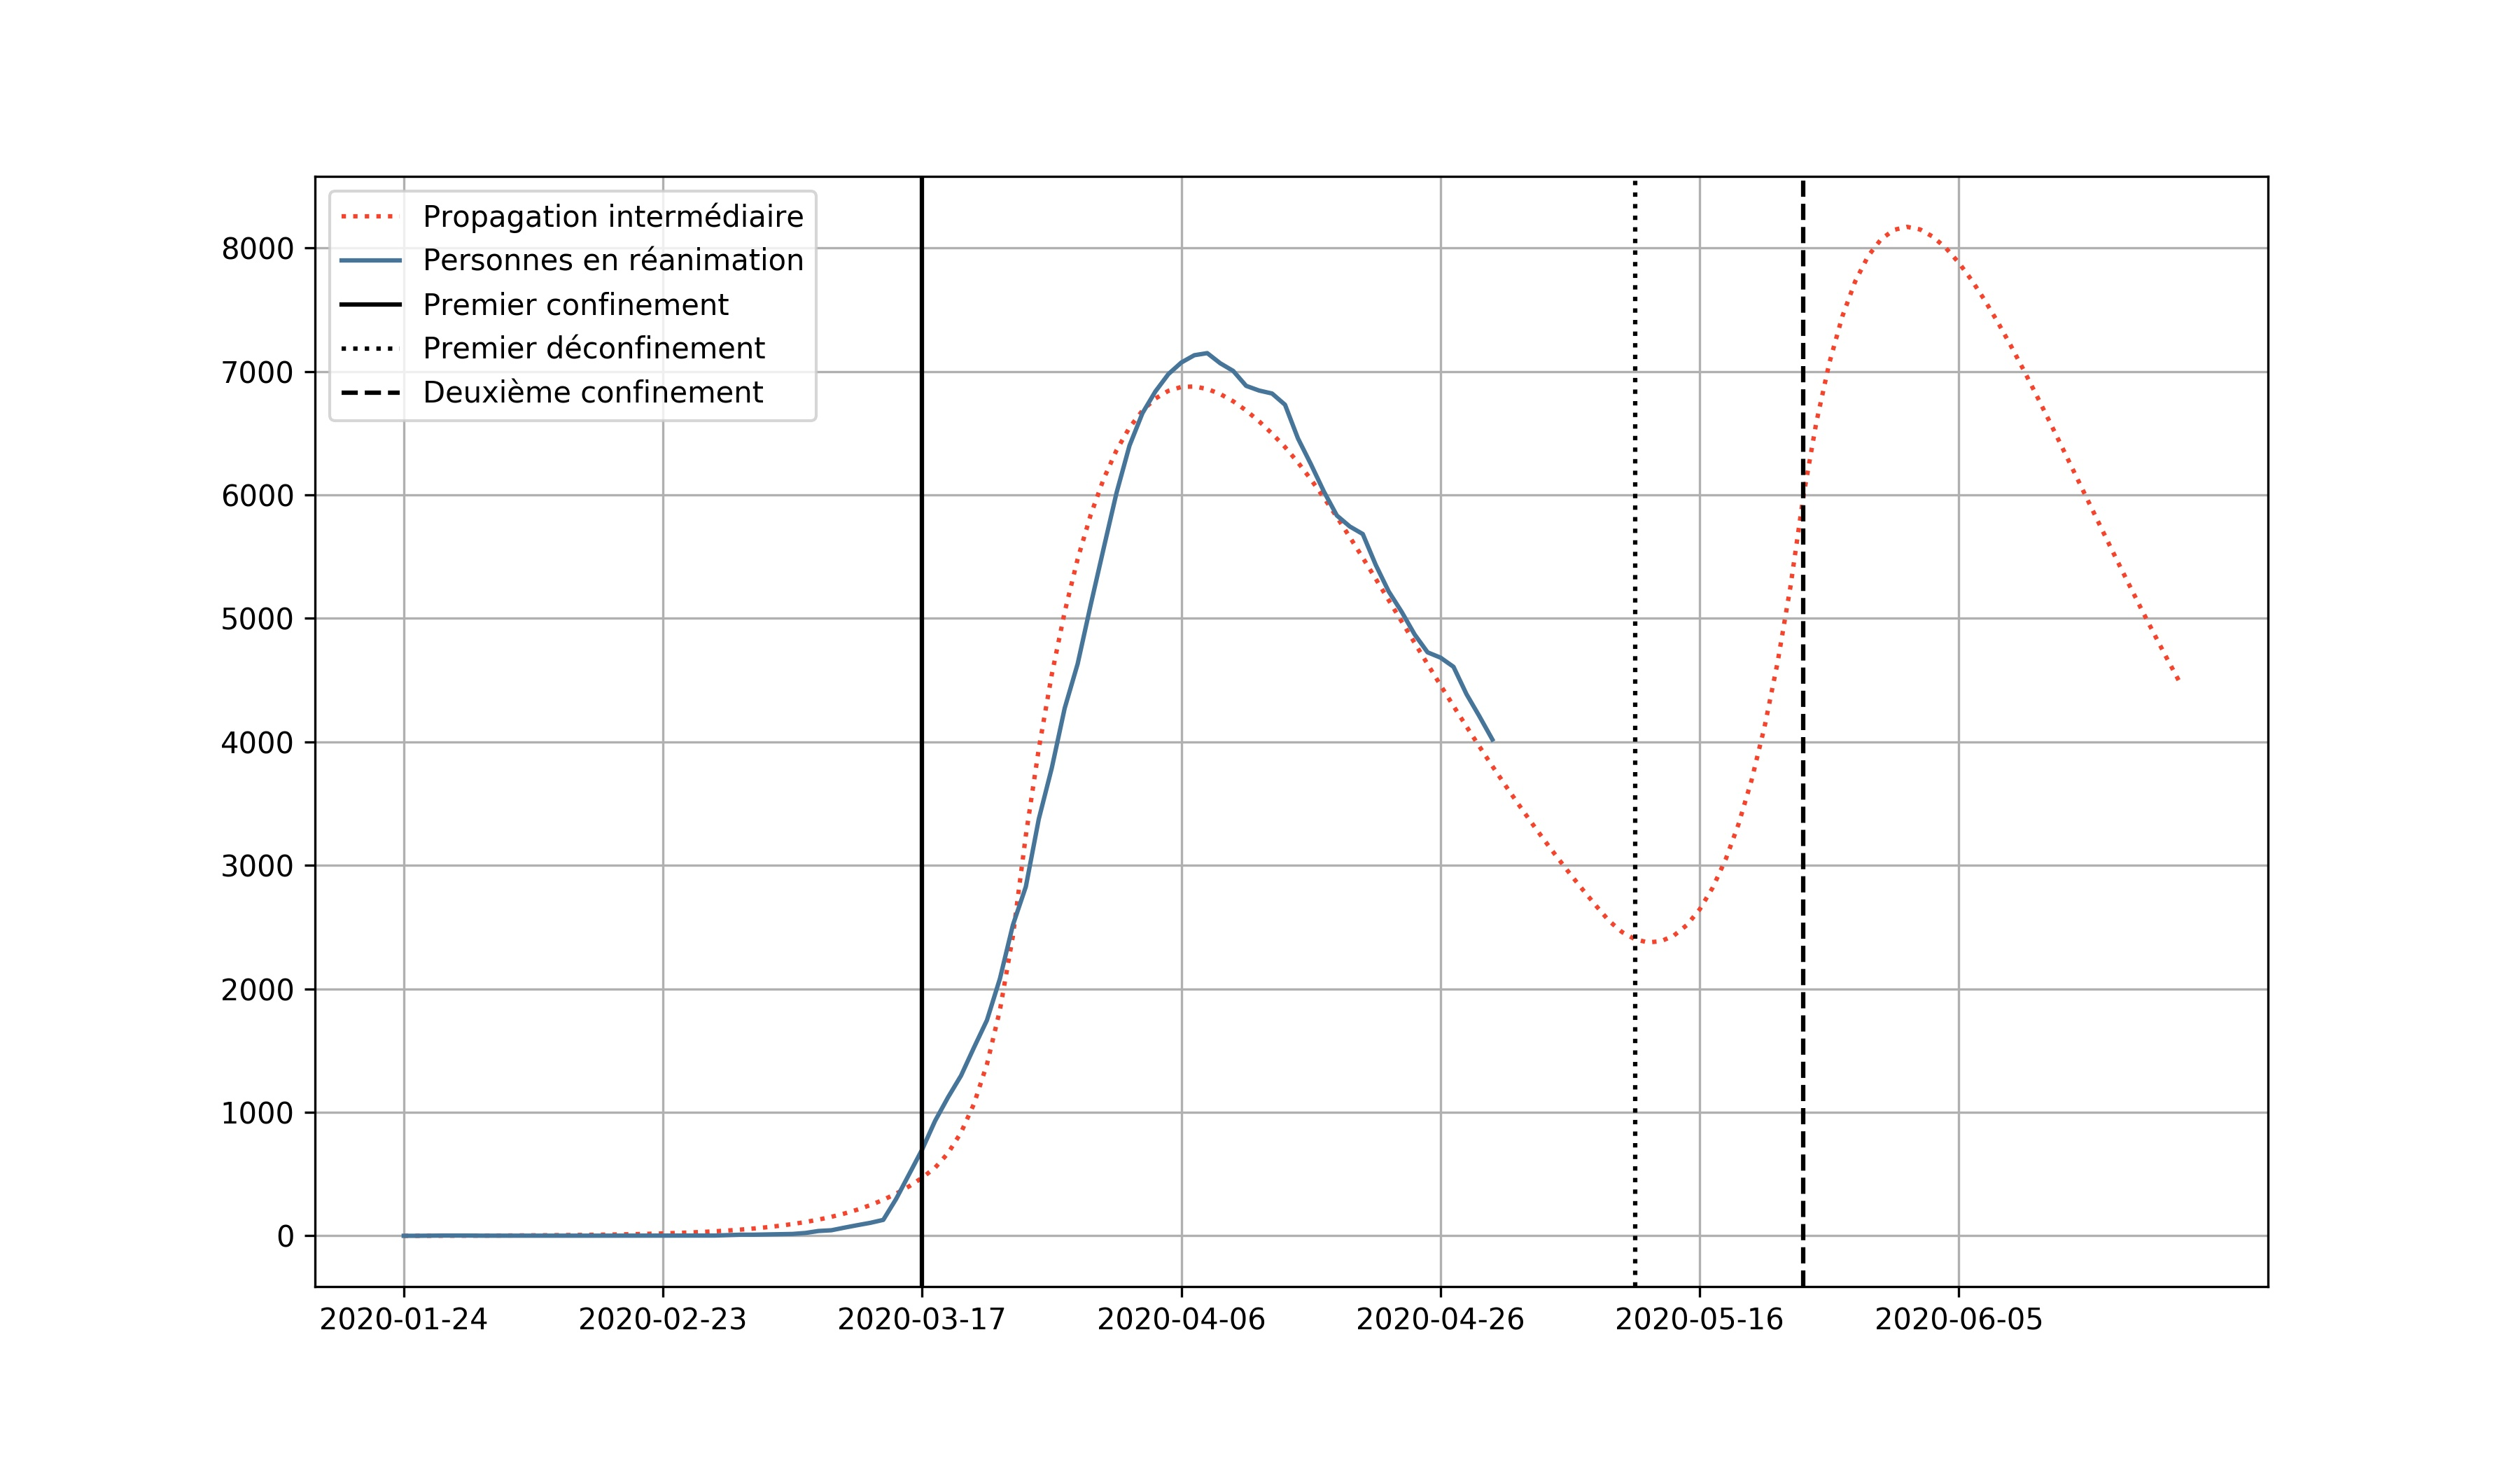
\includegraphics[width=1.0\linewidth]{figure7.jpg} \\

      \textbf{On passe à 8000 Réa !!}
  \end{center}
  
\end{frame}

% --------------------------------------

\begin{frame}[fragile]
\frametitle{Et si le 13 mai on fait légèrement la fête ?}

  \begin{center}
    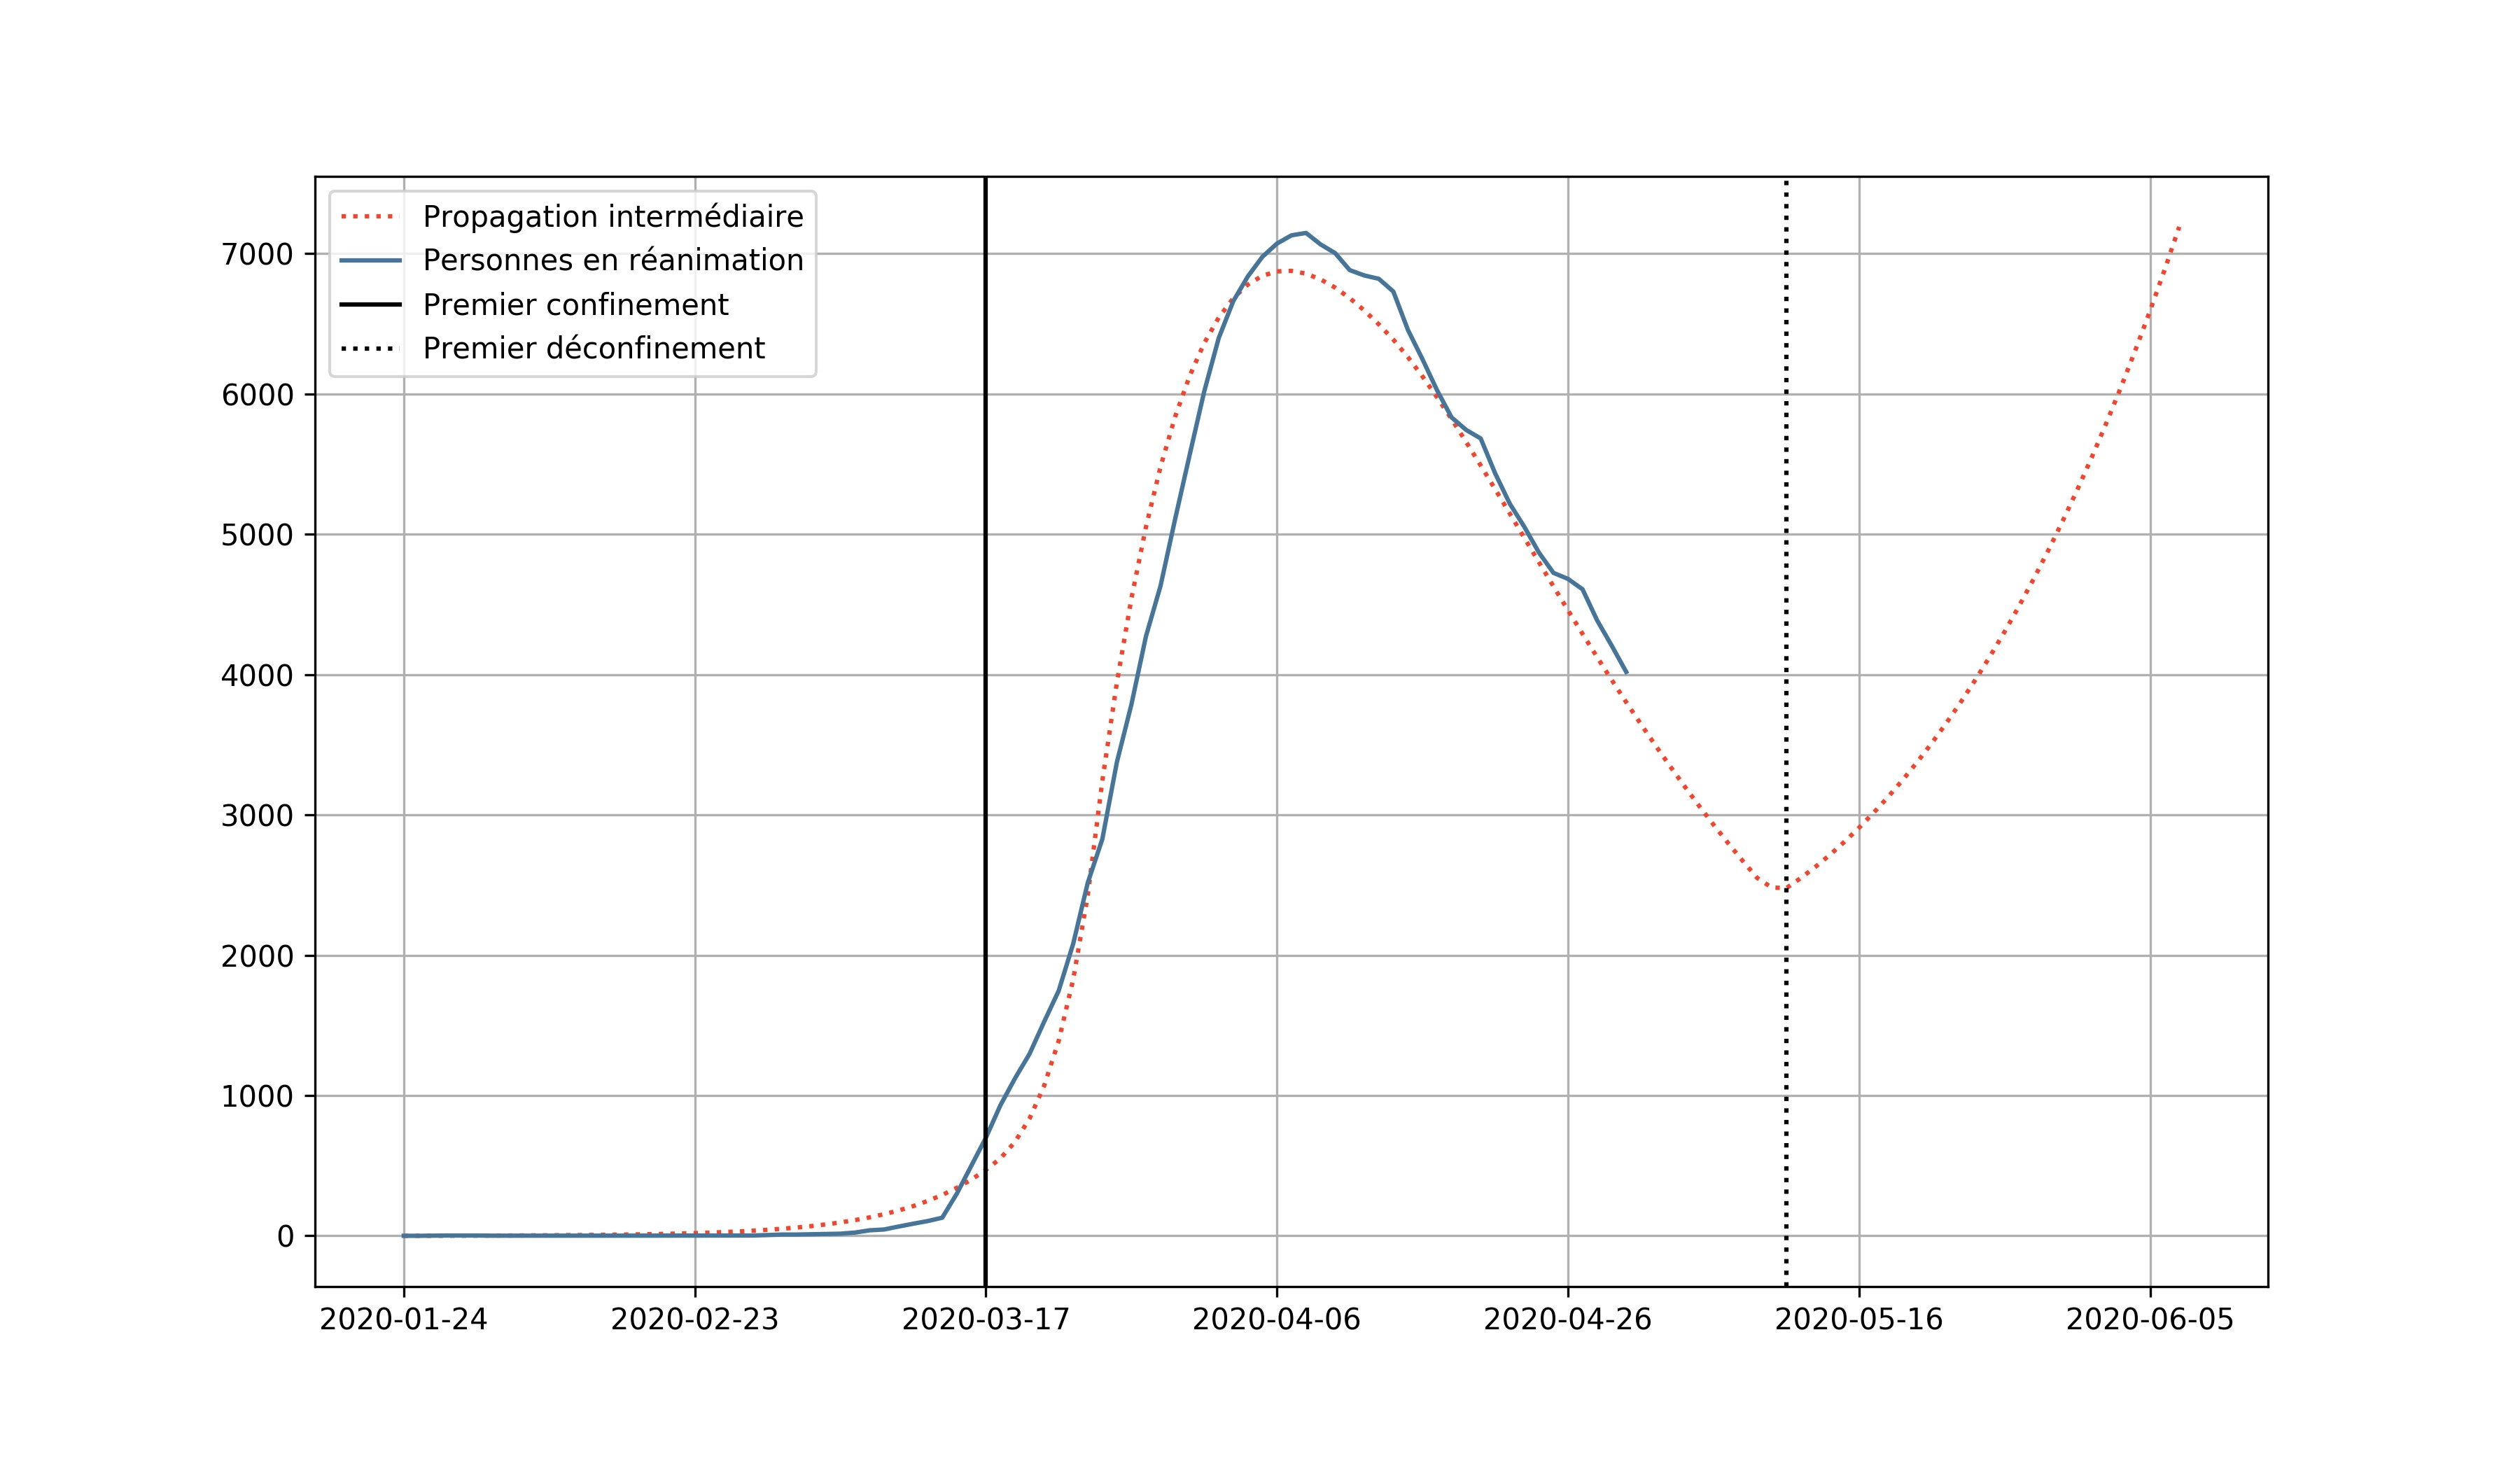
\includegraphics[width=1.0\linewidth]{figure8.jpg} \\
    {\tiny à partir des données ministère santé \texttt{data.gouv.fr}}
  \end{center}
  
\end{frame}




% --------------------------------------

\begin{frame}[fragile]
  \frametitle{Comparaison avec Pasteur}

  \begin{center}
    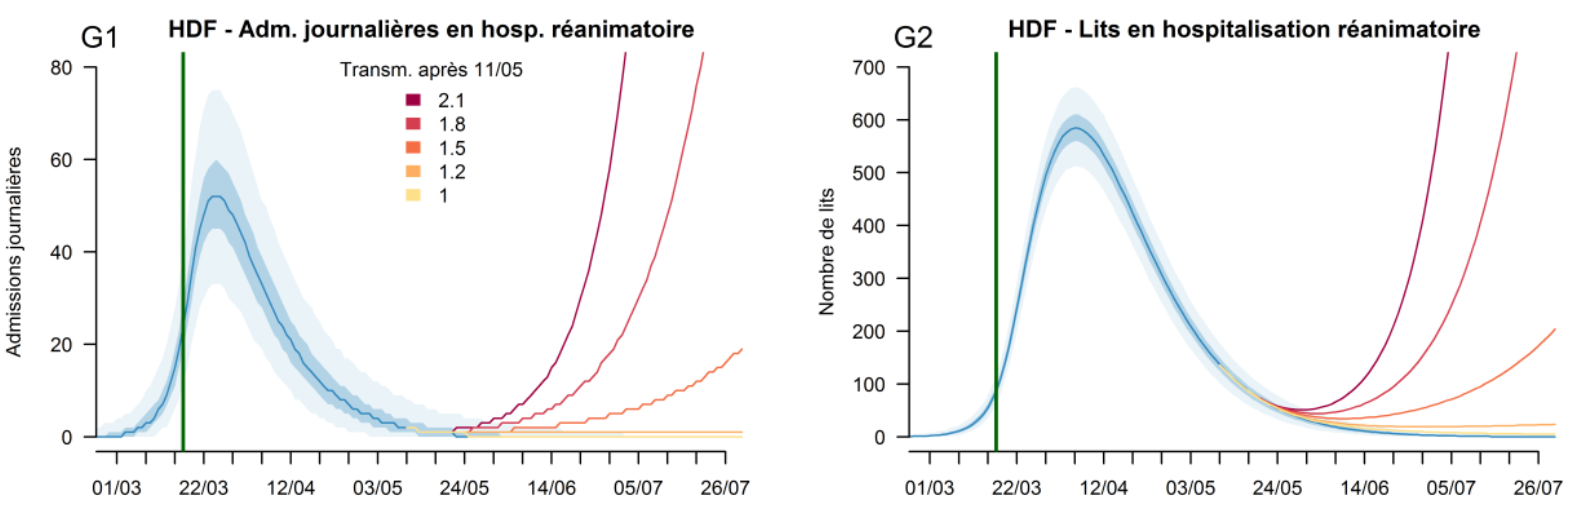
\includegraphics[width=\linewidth]{Inserm+Pasteur_HdF.png}

    {\scriptsize Note 30 du Groupe de modélisation de l’épidémie COVID, 25 avril 2020}
    
  \end{center}

\end{frame}



% --------------------------------------


\begin{frame}
  \hfill \
  \begin{center}
    \Huge
    Conclusion
  \end{center}
  \hfill \

\end{frame}

% --------------------------------------

\begin{frame}[fragile]
  \frametitle{Mise en garde}

  Ne jamais perdre de vue que  :
  \begin{itemize}
  \item Un modèle n'est qu'une abstraction de la réalité
  \item L'important n'est pas d'avoir le plus de paramètres, mais de trouver les plus pertinents (l'essence du problème étudié)
  \item Pour que les thématiciens accaparent un modèle, il faut qu'il soit simple (exemple le modèle SIR : 3 boite cité dans des centaines de travaux en épidémio)
  \end{itemize}

  \bigskip
  
  \begin{block}{}
    \begin{center}
  Torturez un modèle, il finit toujours par avouer !
\end{center}
\end{block}

\end{frame}

% --------------------------------------

\begin{frame}[fragile]
  \frametitle{Nous sommes complémentaires !}

  \begin{itemize}
  \item Notre modèle est adaptable en tout point
  \item Il y a surement plein de biais .... \\ Nous avons besoin de
    collaborer
  \end{itemize}

  \bigskip

  
  \begin{itemize}
    \item Nous sommes juste des modélisateurs
    \item Nous avons besoin de votre experience de spécialistes
    \item Qu'est-ce que vous attendez de nous ?
    \end{itemize}

  
\end{frame}


\end{document}

